\section{Entropic Regularization of Optimal Transport}

This tour focused on the entropic regularization of the original optimal transport problem. Considering two discrete distributions $a,b \in \Sigma_n$, the Kantorovitch formulation reads: 
\begin{equation*}
    W(a,b) \eqdef \umin{P \in U(a,b)} \dotp{C}{P} 
\end{equation*}
Whereas the entropic regularization reads:
\begin{equation*}
    W_\epsilon(a,b) \eqdef \umin{P \in U(a,b)} \dotp{C}{P} - \epsilon H(P)
\end{equation*}
Where $H$ is the entropy associated to the coupling $P$:
\begin{equation*}
    H(P) = \sumij P_{ij} \p{\log(P_{i,j}) - 1}
\end{equation*}
and $\epsilon$ is the strenght of this regularization parameter. The problem remains convex, we can show it amounts to taking the Kullback Leibler projection of the Gibbs kernel $K_{ij} = e^{-C_{ij}/\epsilon}$ on $U(a,b)$, and that the smaller the $\epsilon$, the sparser the optimal coupling is and the closer it is from the optimal coupling related to the Kantorovitch formulation. 

\begin{table}[h]
\centering
\begin{tabular}{cc}
\textbf{Small $\epsilon$}      & \textbf{Big $\epsilon$}        \\ \hline
Sparse solution                & Dense solution                 \\ 
Slow convergence               & Fast convergence               \\ 
Close to the unrelaxed problem & Far from the unrelaxed problem \\ 
\end{tabular}
\end{table}

That being said, let's see what this Numerical tour focused on.

\subsection{Transport between point clouds}

We first consider the case of transporting two point clouds. For that part, we keep the data suggested by the notebook, shown fig \ref{fig:two_point_cloud}. 

\begin{figure}[h]
    \centering
    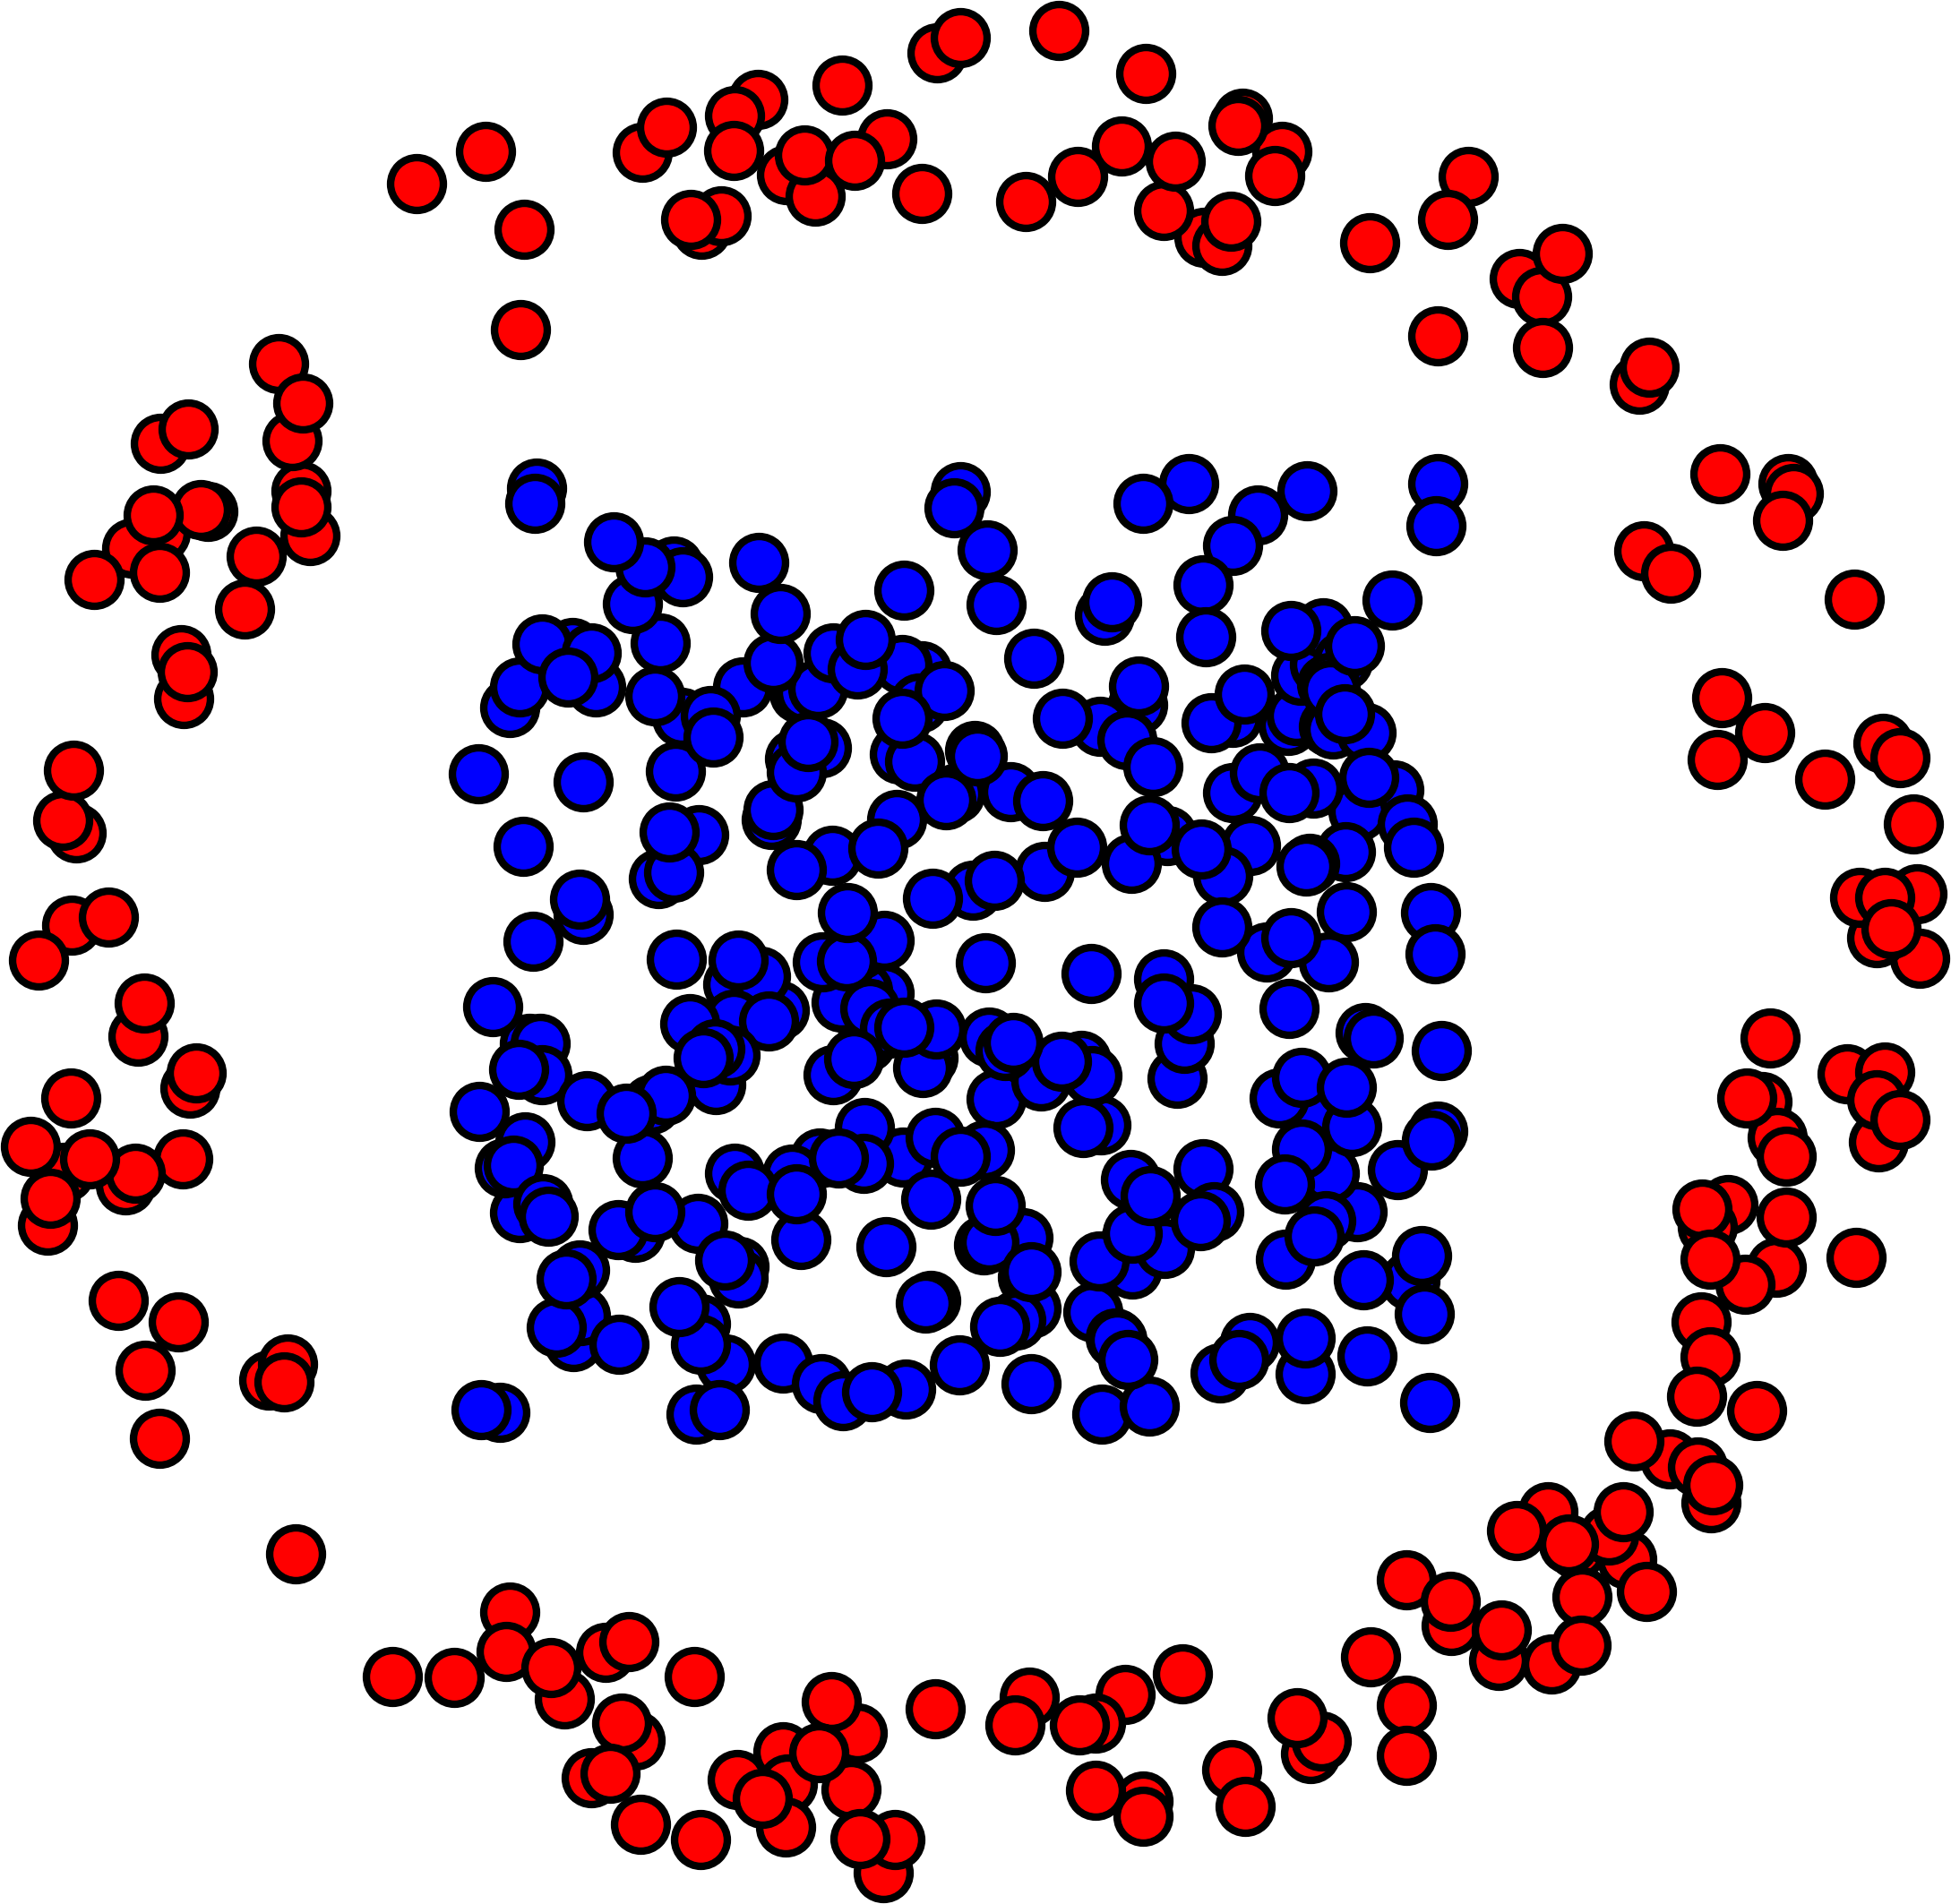
\includegraphics[width=.5\linewidth]{samples/2/two_point_clouds.png}
    \caption{The point clouds we will transport. }
    \label{fig:two_point_cloud}
\end{figure}

We then implement the Sinkhorn's algorithm to solve the transport plan. The implementation is straightforward, as it only requires applying the update on the dual variable and iterating until a minimum tolerance for the equality constraints or a maximum number of iteration has been reached. One can refer to the notebook for the code. 

\subsubsection{Speed of convergence}

We first check the \textbf{influence of $\epsilon$ on the convergence of the algorithm}. There is a trade off here between fast convergence and closeness to Kantorovitch solution. This is shown on fig. \ref{fig:violation_eps}.

\begin{figure}[h]
    \centering
    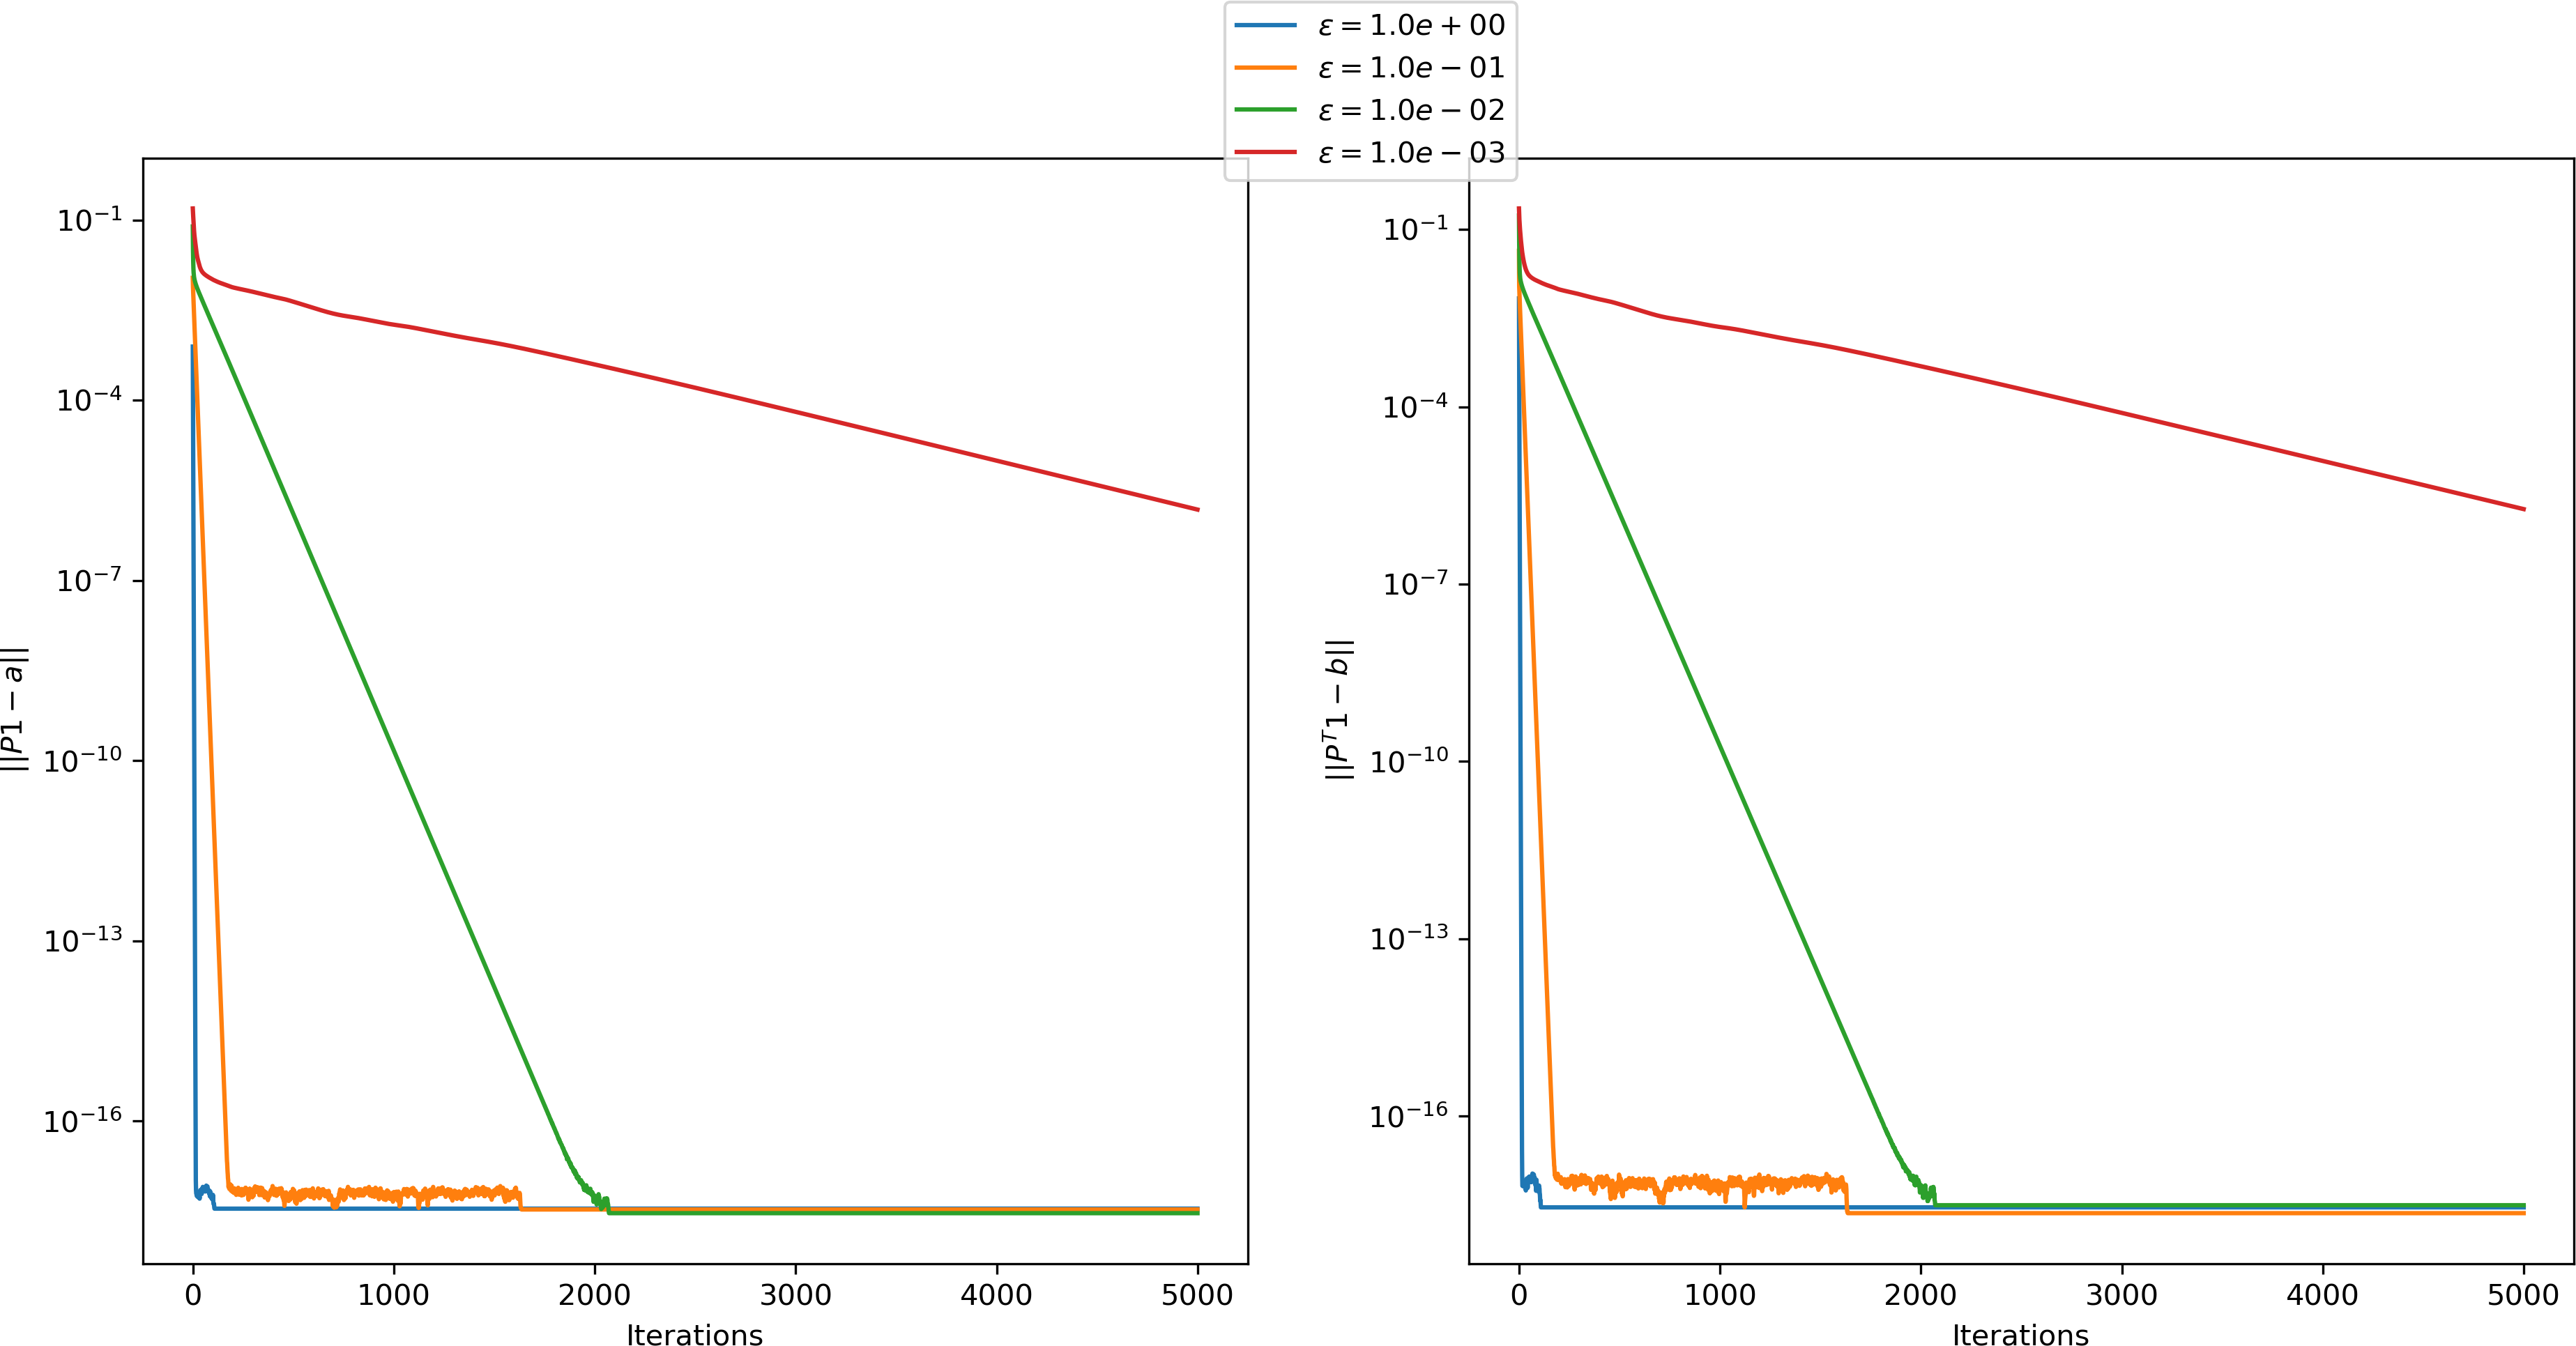
\includegraphics[width=1\textwidth]{samples/2/violation_eps.png}
    \caption{Speed of convergence function of $\epsilon$.}
    \label{fig:violation_eps}
\end{figure}

We check our precedent statement. When $\epsilon$ is close to 1, we reach very quickly machine precision, whereas the slop is smaller as $\epsilon$ decreases. This behaviour is visible on the next plot, where we show the number of iterations needed to reach a certain precision function of $\epsilon$ value (fig. \ref{fig:iteration_function_of_eps}).

\begin{figure}[h]
    \centering
    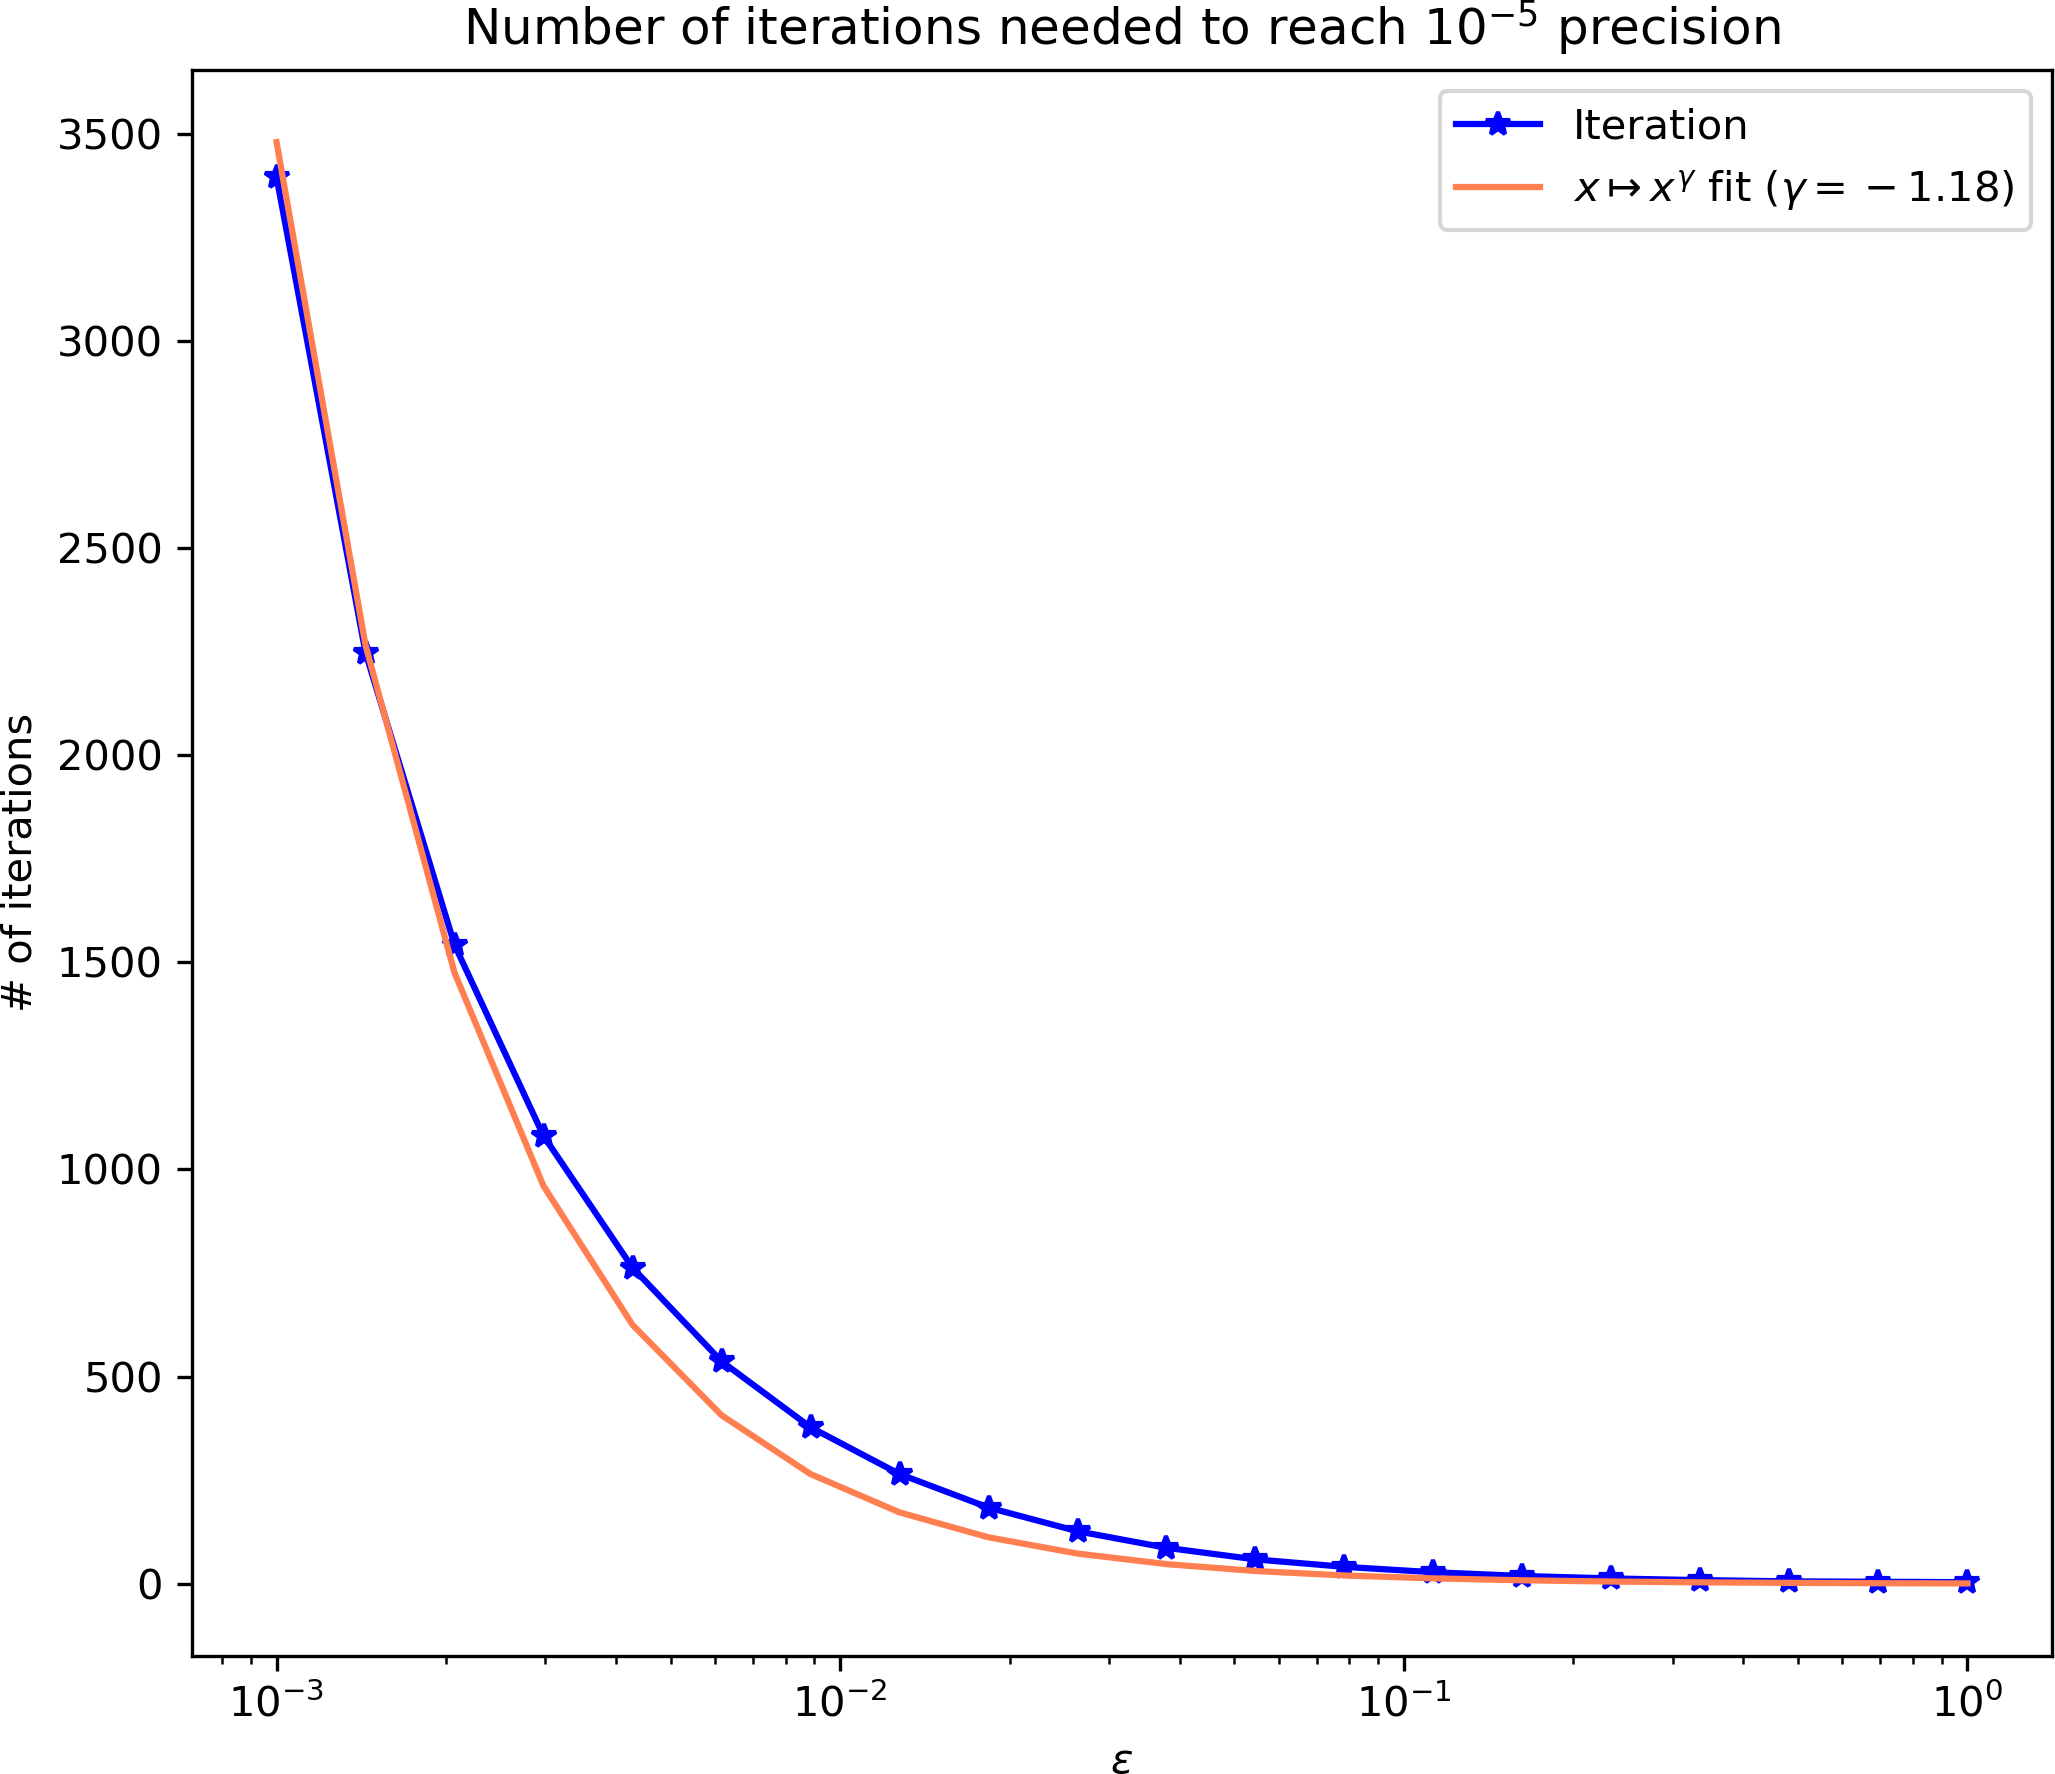
\includegraphics[width=.7\textwidth]{samples/2/iteration_function_of_eps.png}
    \caption{Number of iterations needed to reach a precision of $10^{-5}$, function of $\epsilon$. A polynomial fit is shown for information (obtained via least squares).}
    \label{fig:iteration_function_of_eps}
\end{figure}

Interestingly, if $\epsilon$ is too low (I found $4 10^{-4}$ to be the limit), the algorithm \textbf{never converges}. This is simply because the Gibbs kernel gets huge and overflows, and this can be addressed by making the computations in the \textbf{log domain}. 

\subsubsection{Sparsity of the coupling}

Let's now check the sparsity of the coupling. A visual is provided fig. \ref{fig:coupling_function_of_eps}.

\begin{figure}[h]
    \centering
    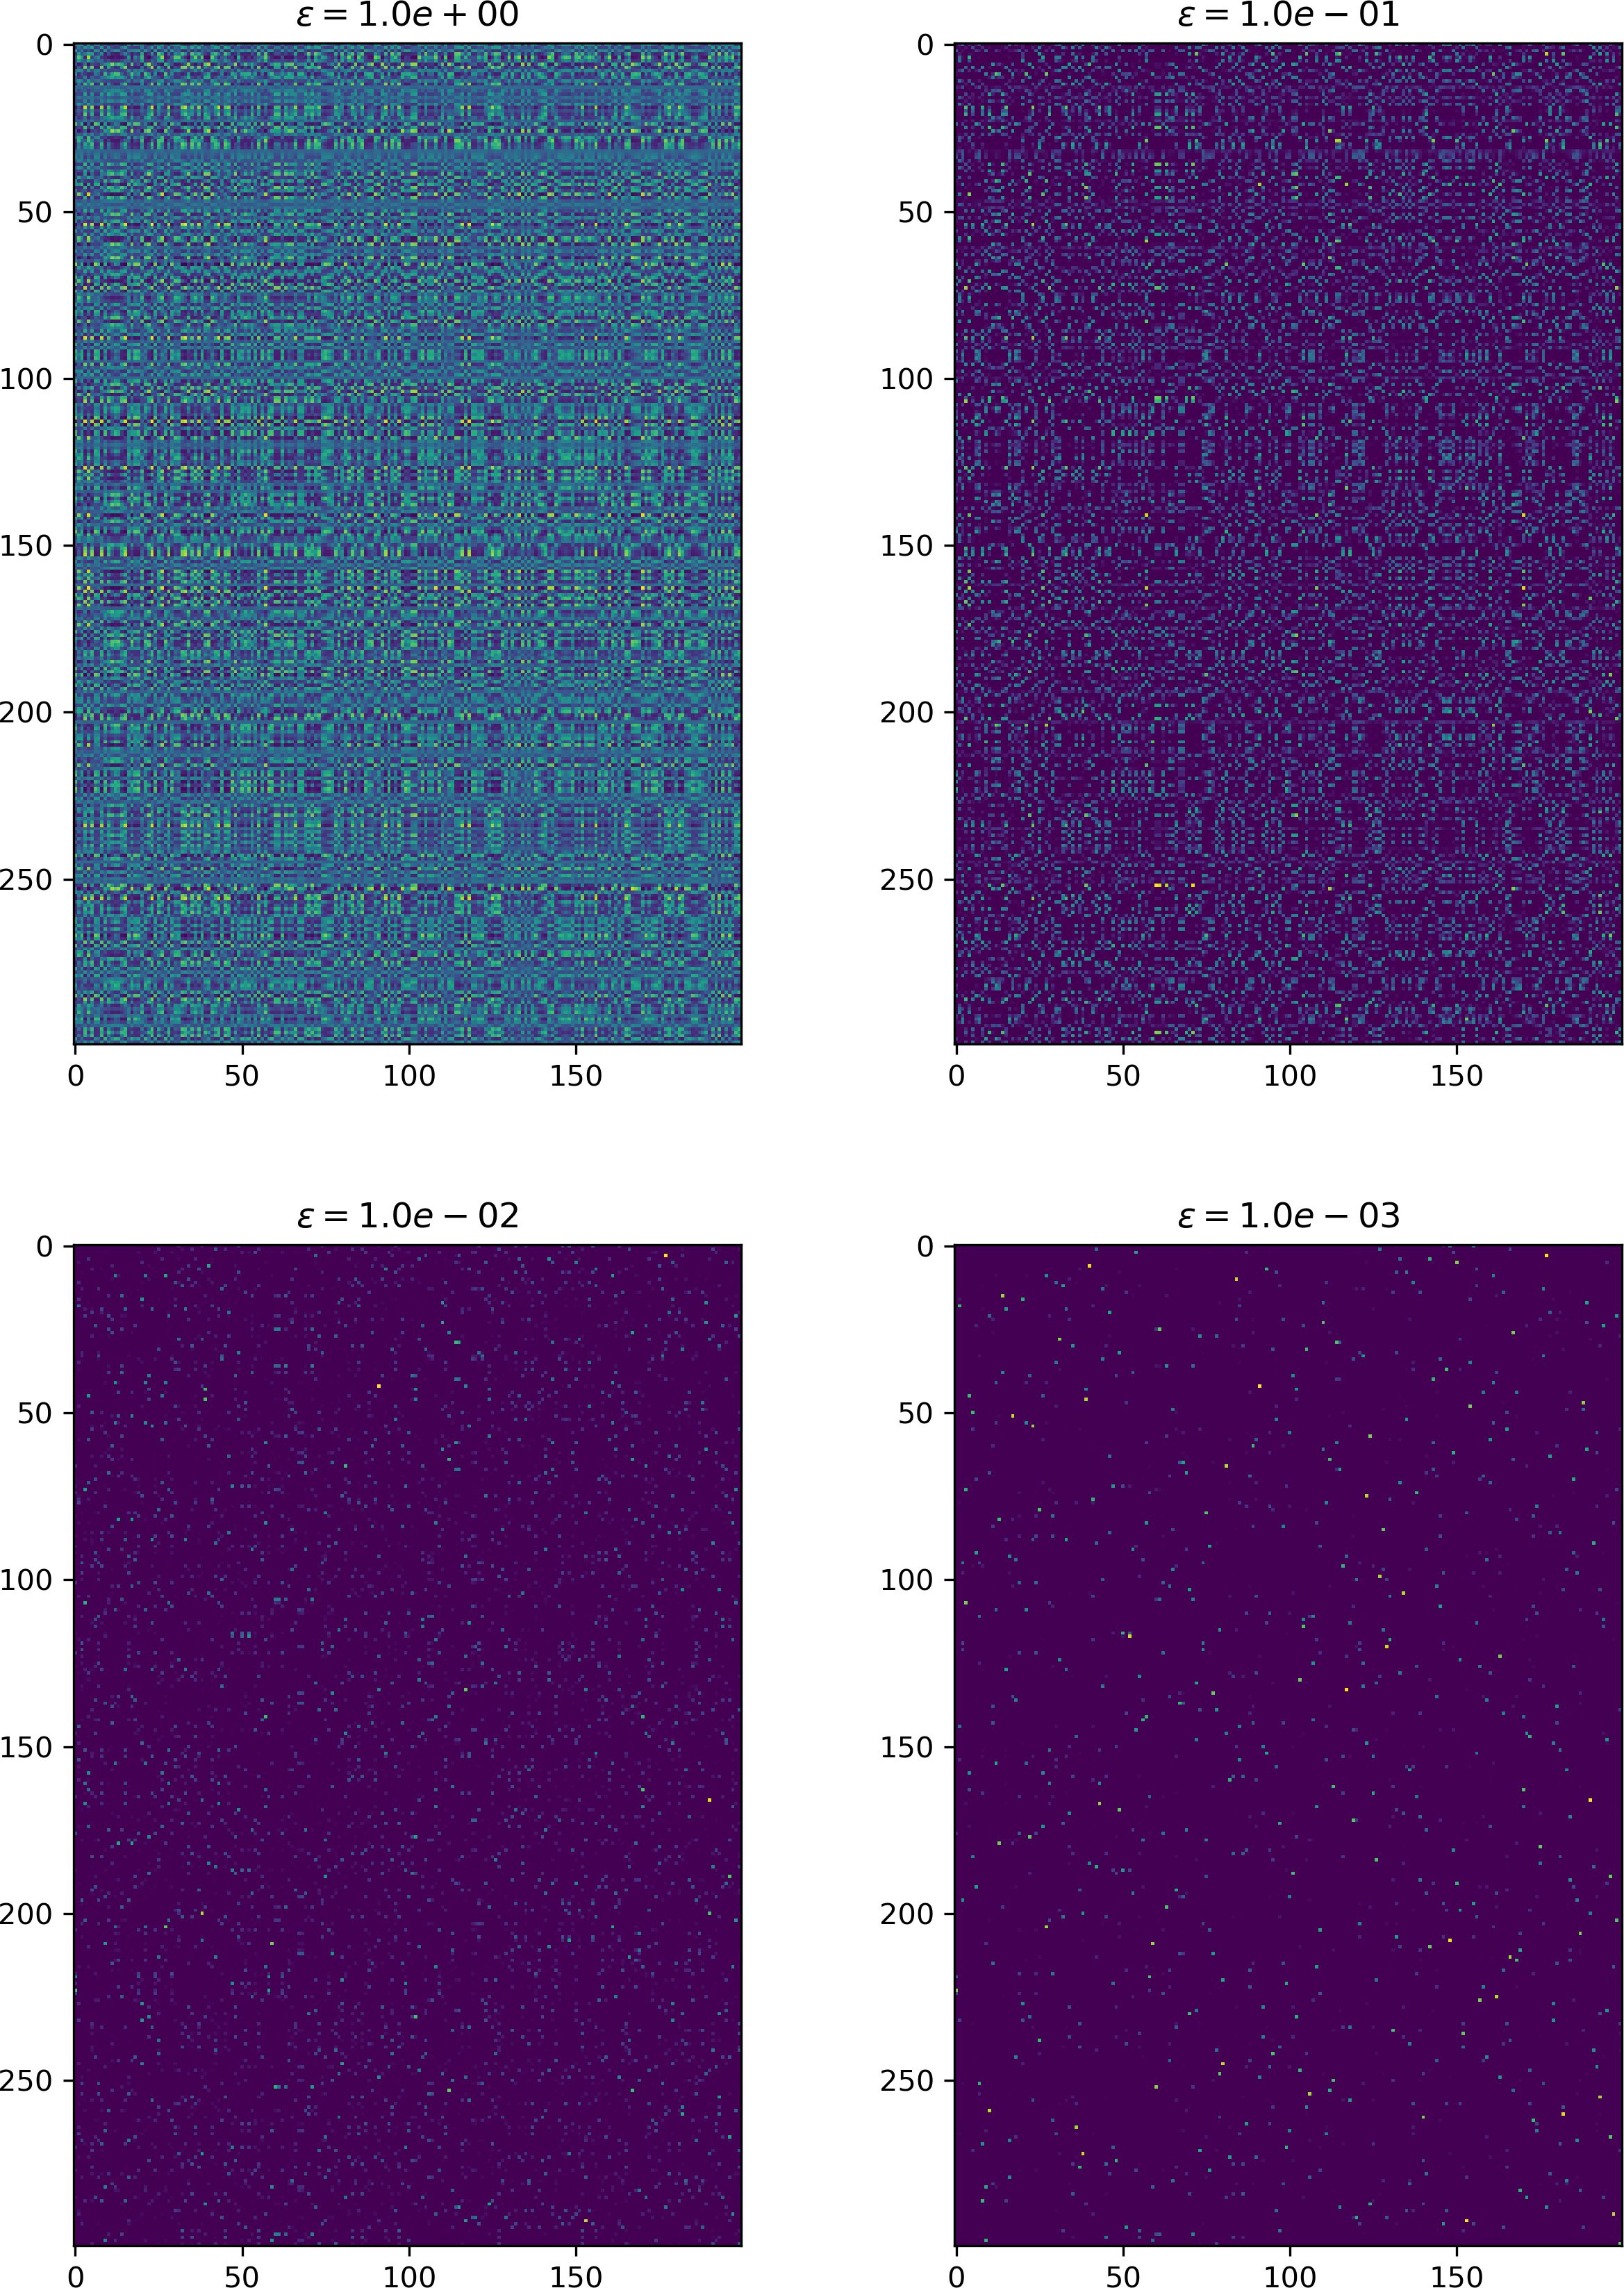
\includegraphics[width=.7\linewidth]{samples/2/coupling_function_of_eps.png}
    \caption{Coupling matrix $P$ for various values of $\epsilon$.}
    \label{fig:coupling_function_of_eps}
\end{figure}

The higher epsilon, the denser the coupling. We can choose to plot the number of non-zero entries, function of $\epsilon$. This is shown fig. \ref{fig:fraction_null}.

\begin{figure}[h]
    \centering
    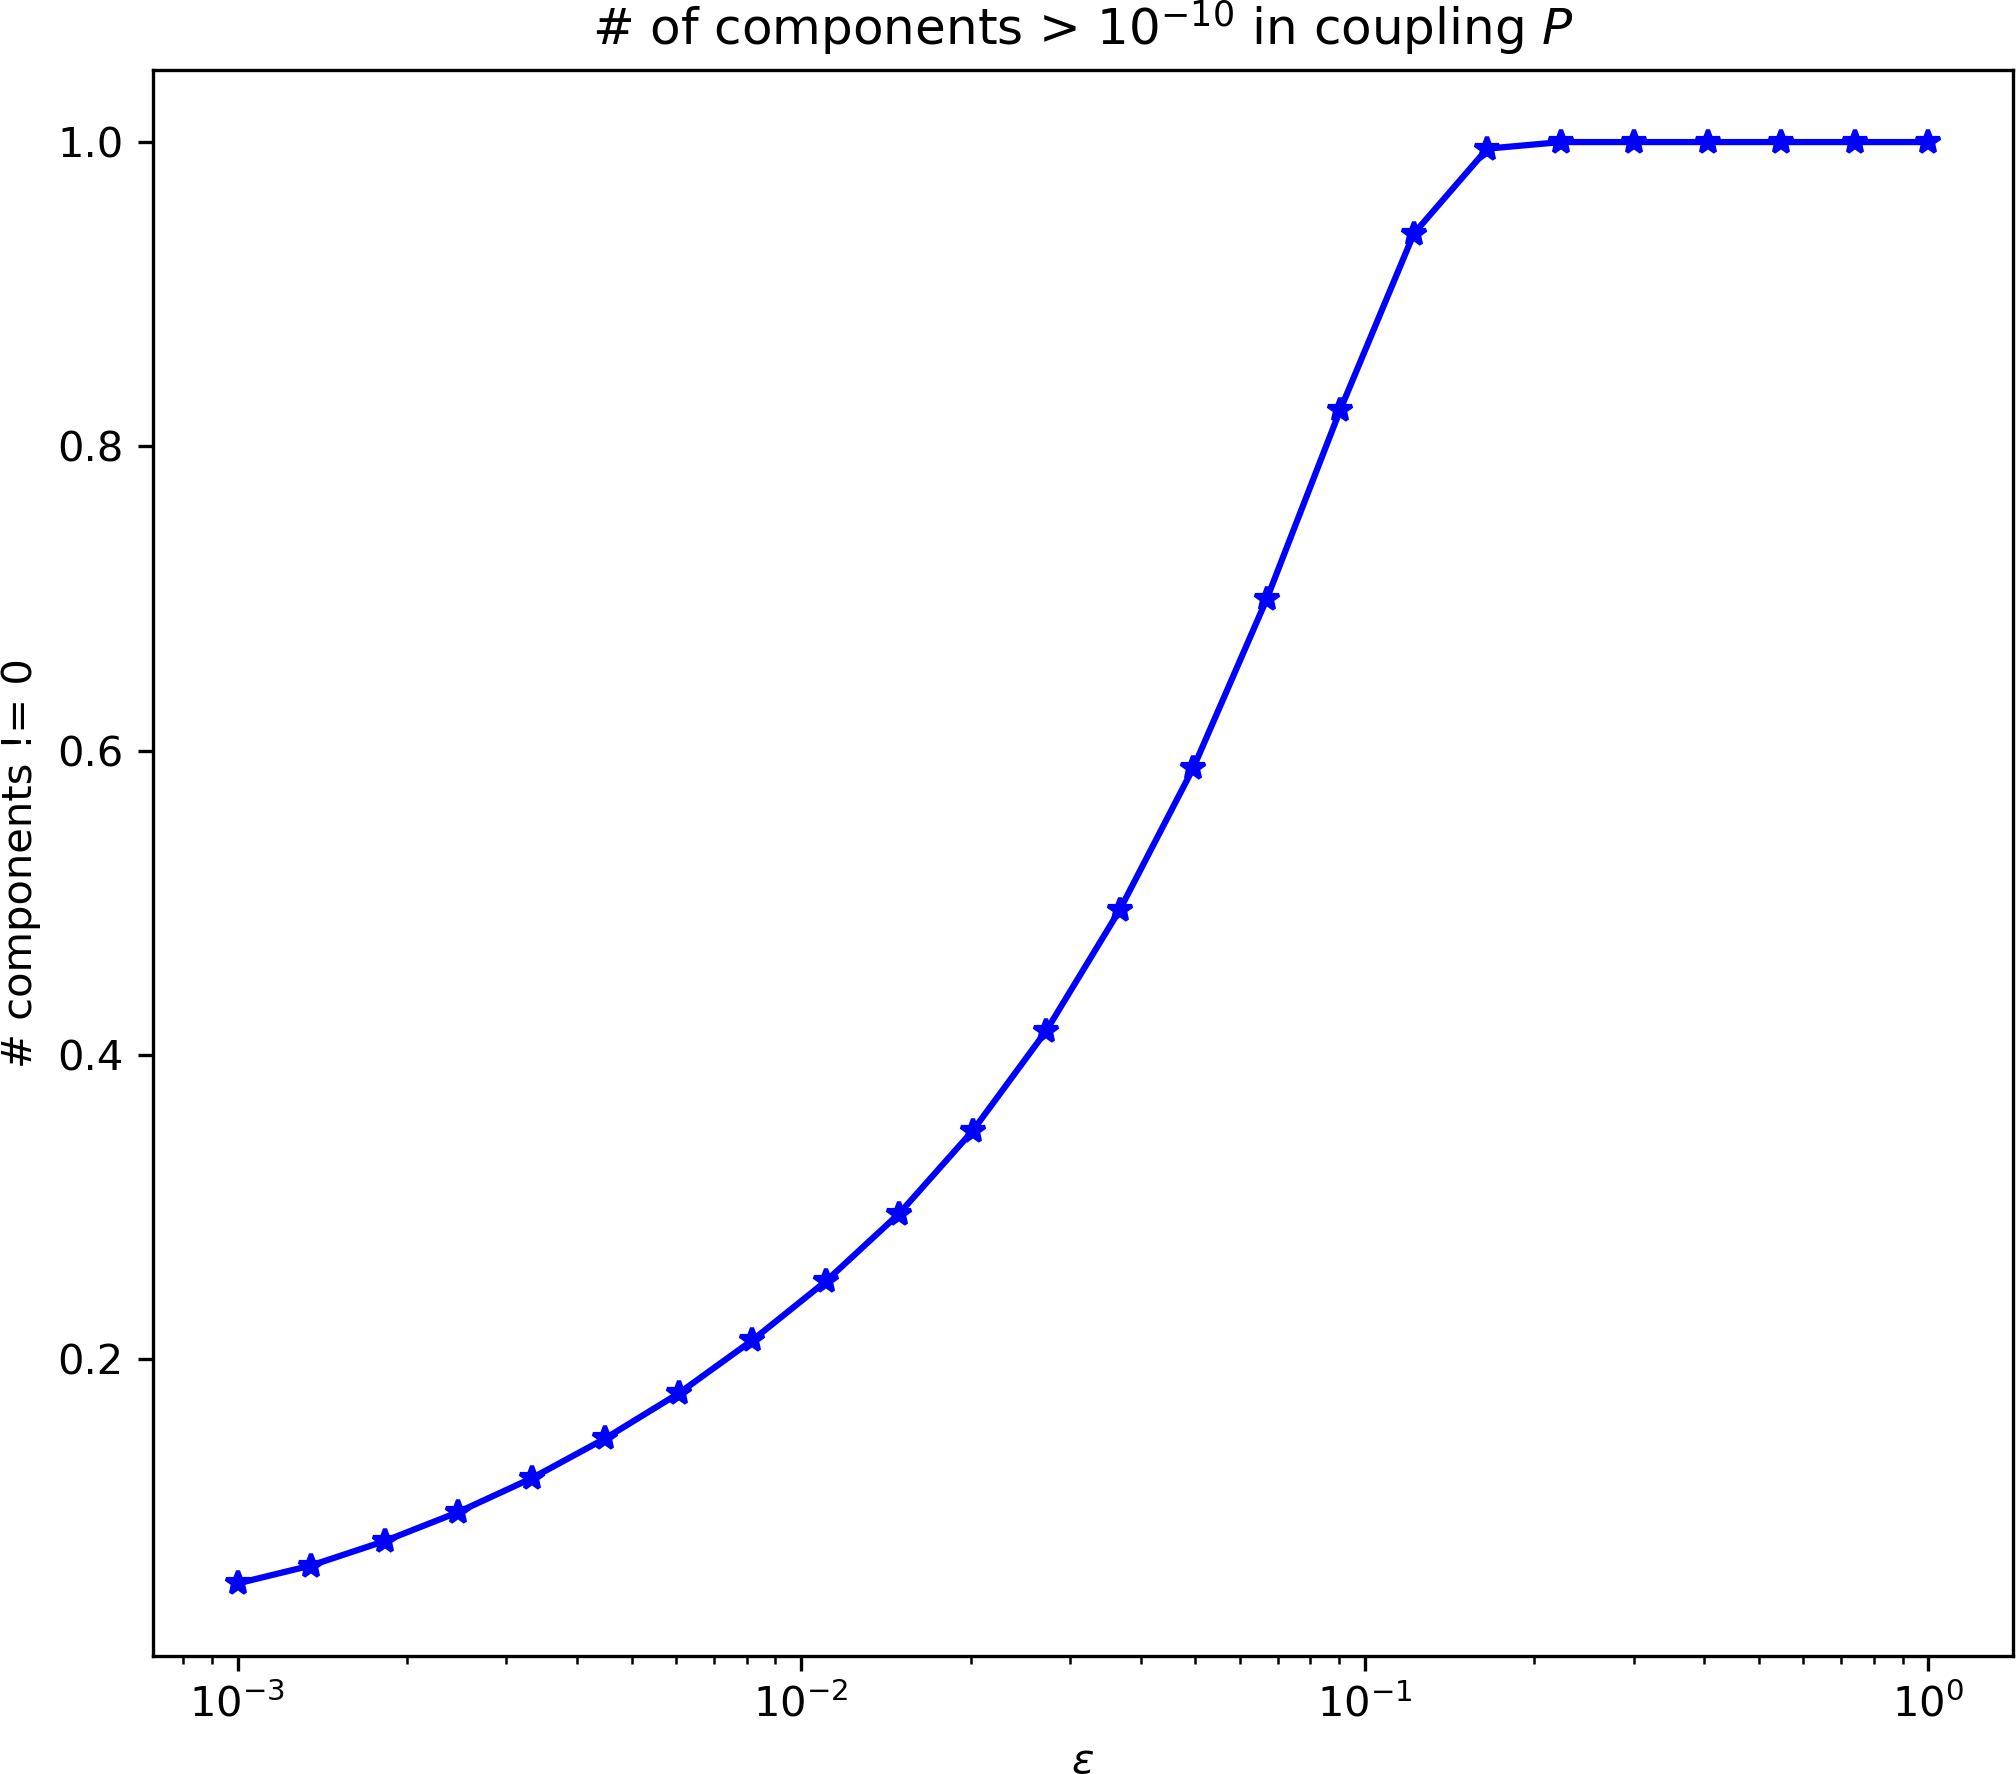
\includegraphics[width=.7\textwidth]{samples/2/fraction_null_components.png}
    \caption{Fraction of non-zero components, function of $\epsilon$.}
    \label{fig:fraction_null}
\end{figure}

Finally, a more visual interpretation is provided fig. \ref{fig:coupling_eps}.

\begin{figure}[h]
     \centering
     \begin{subfigure}[t]{0.49\textwidth}
         \centering
         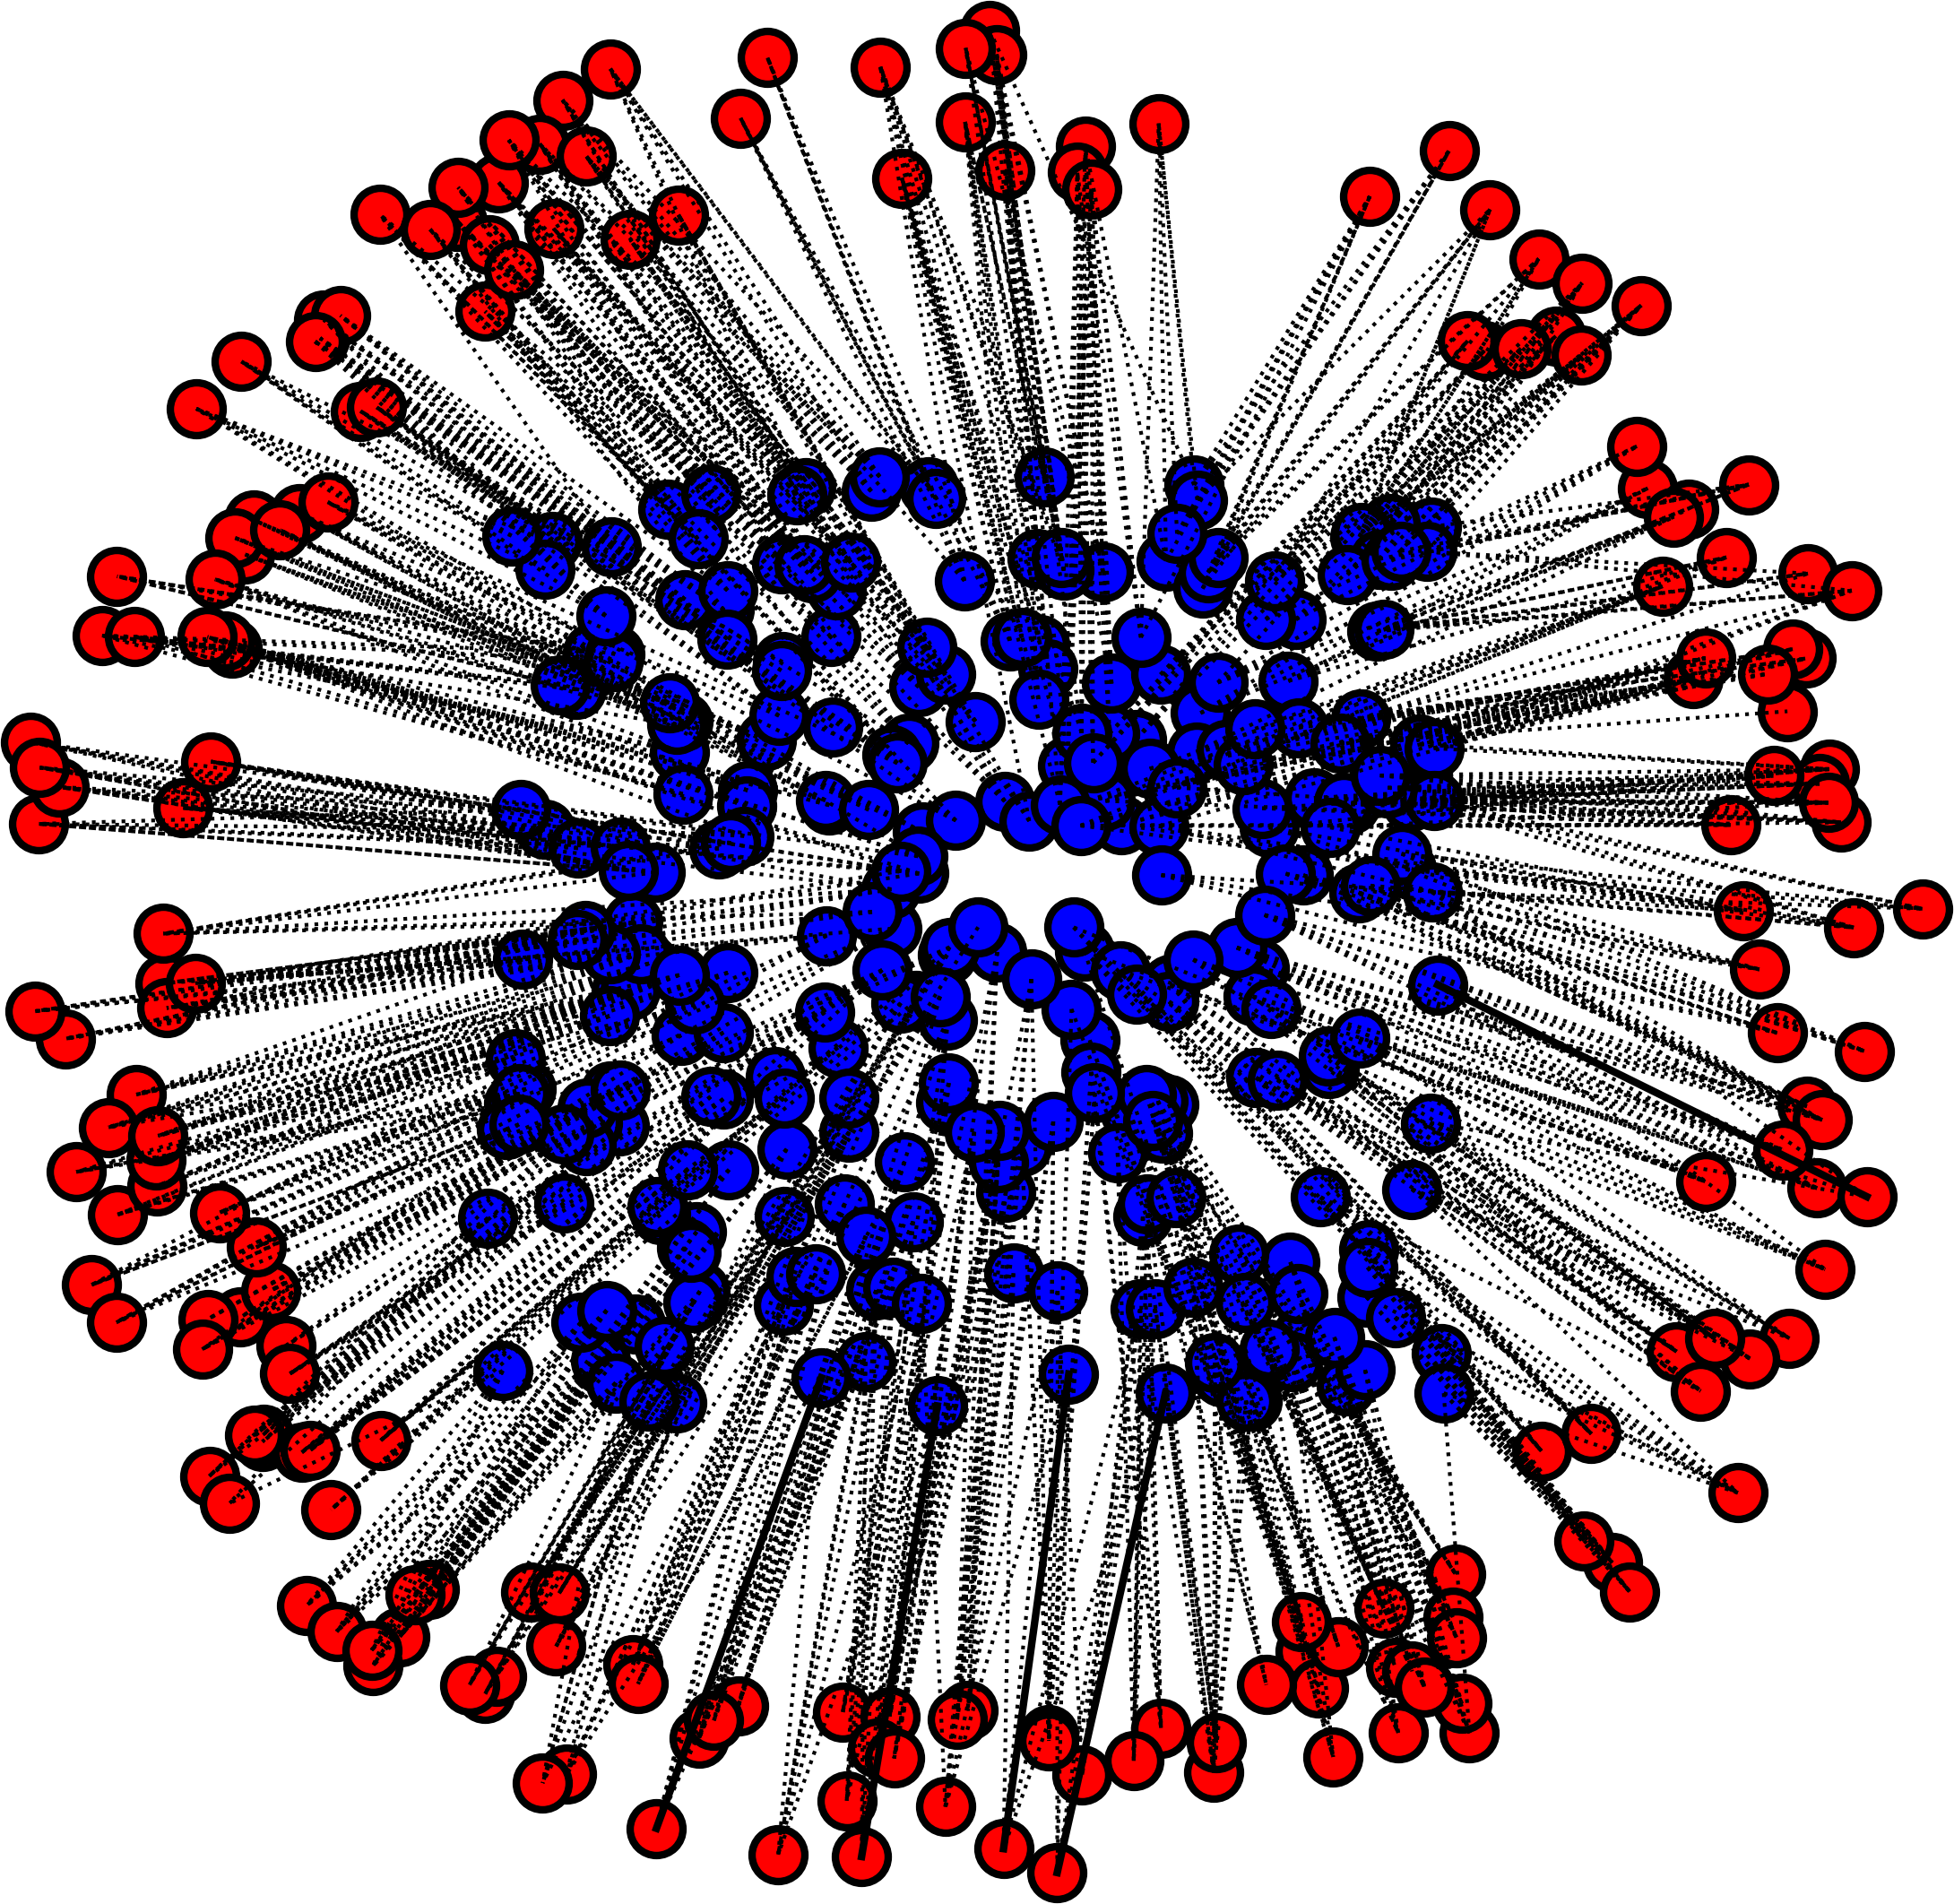
\includegraphics[width=\textwidth]{samples/2/coupling_eps_1e-2.png}
         \caption{$\epsilon=\tenp{-2}$}
     \end{subfigure}
     \hfill
     \begin{subfigure}[t]{0.49\textwidth}
         \centering
         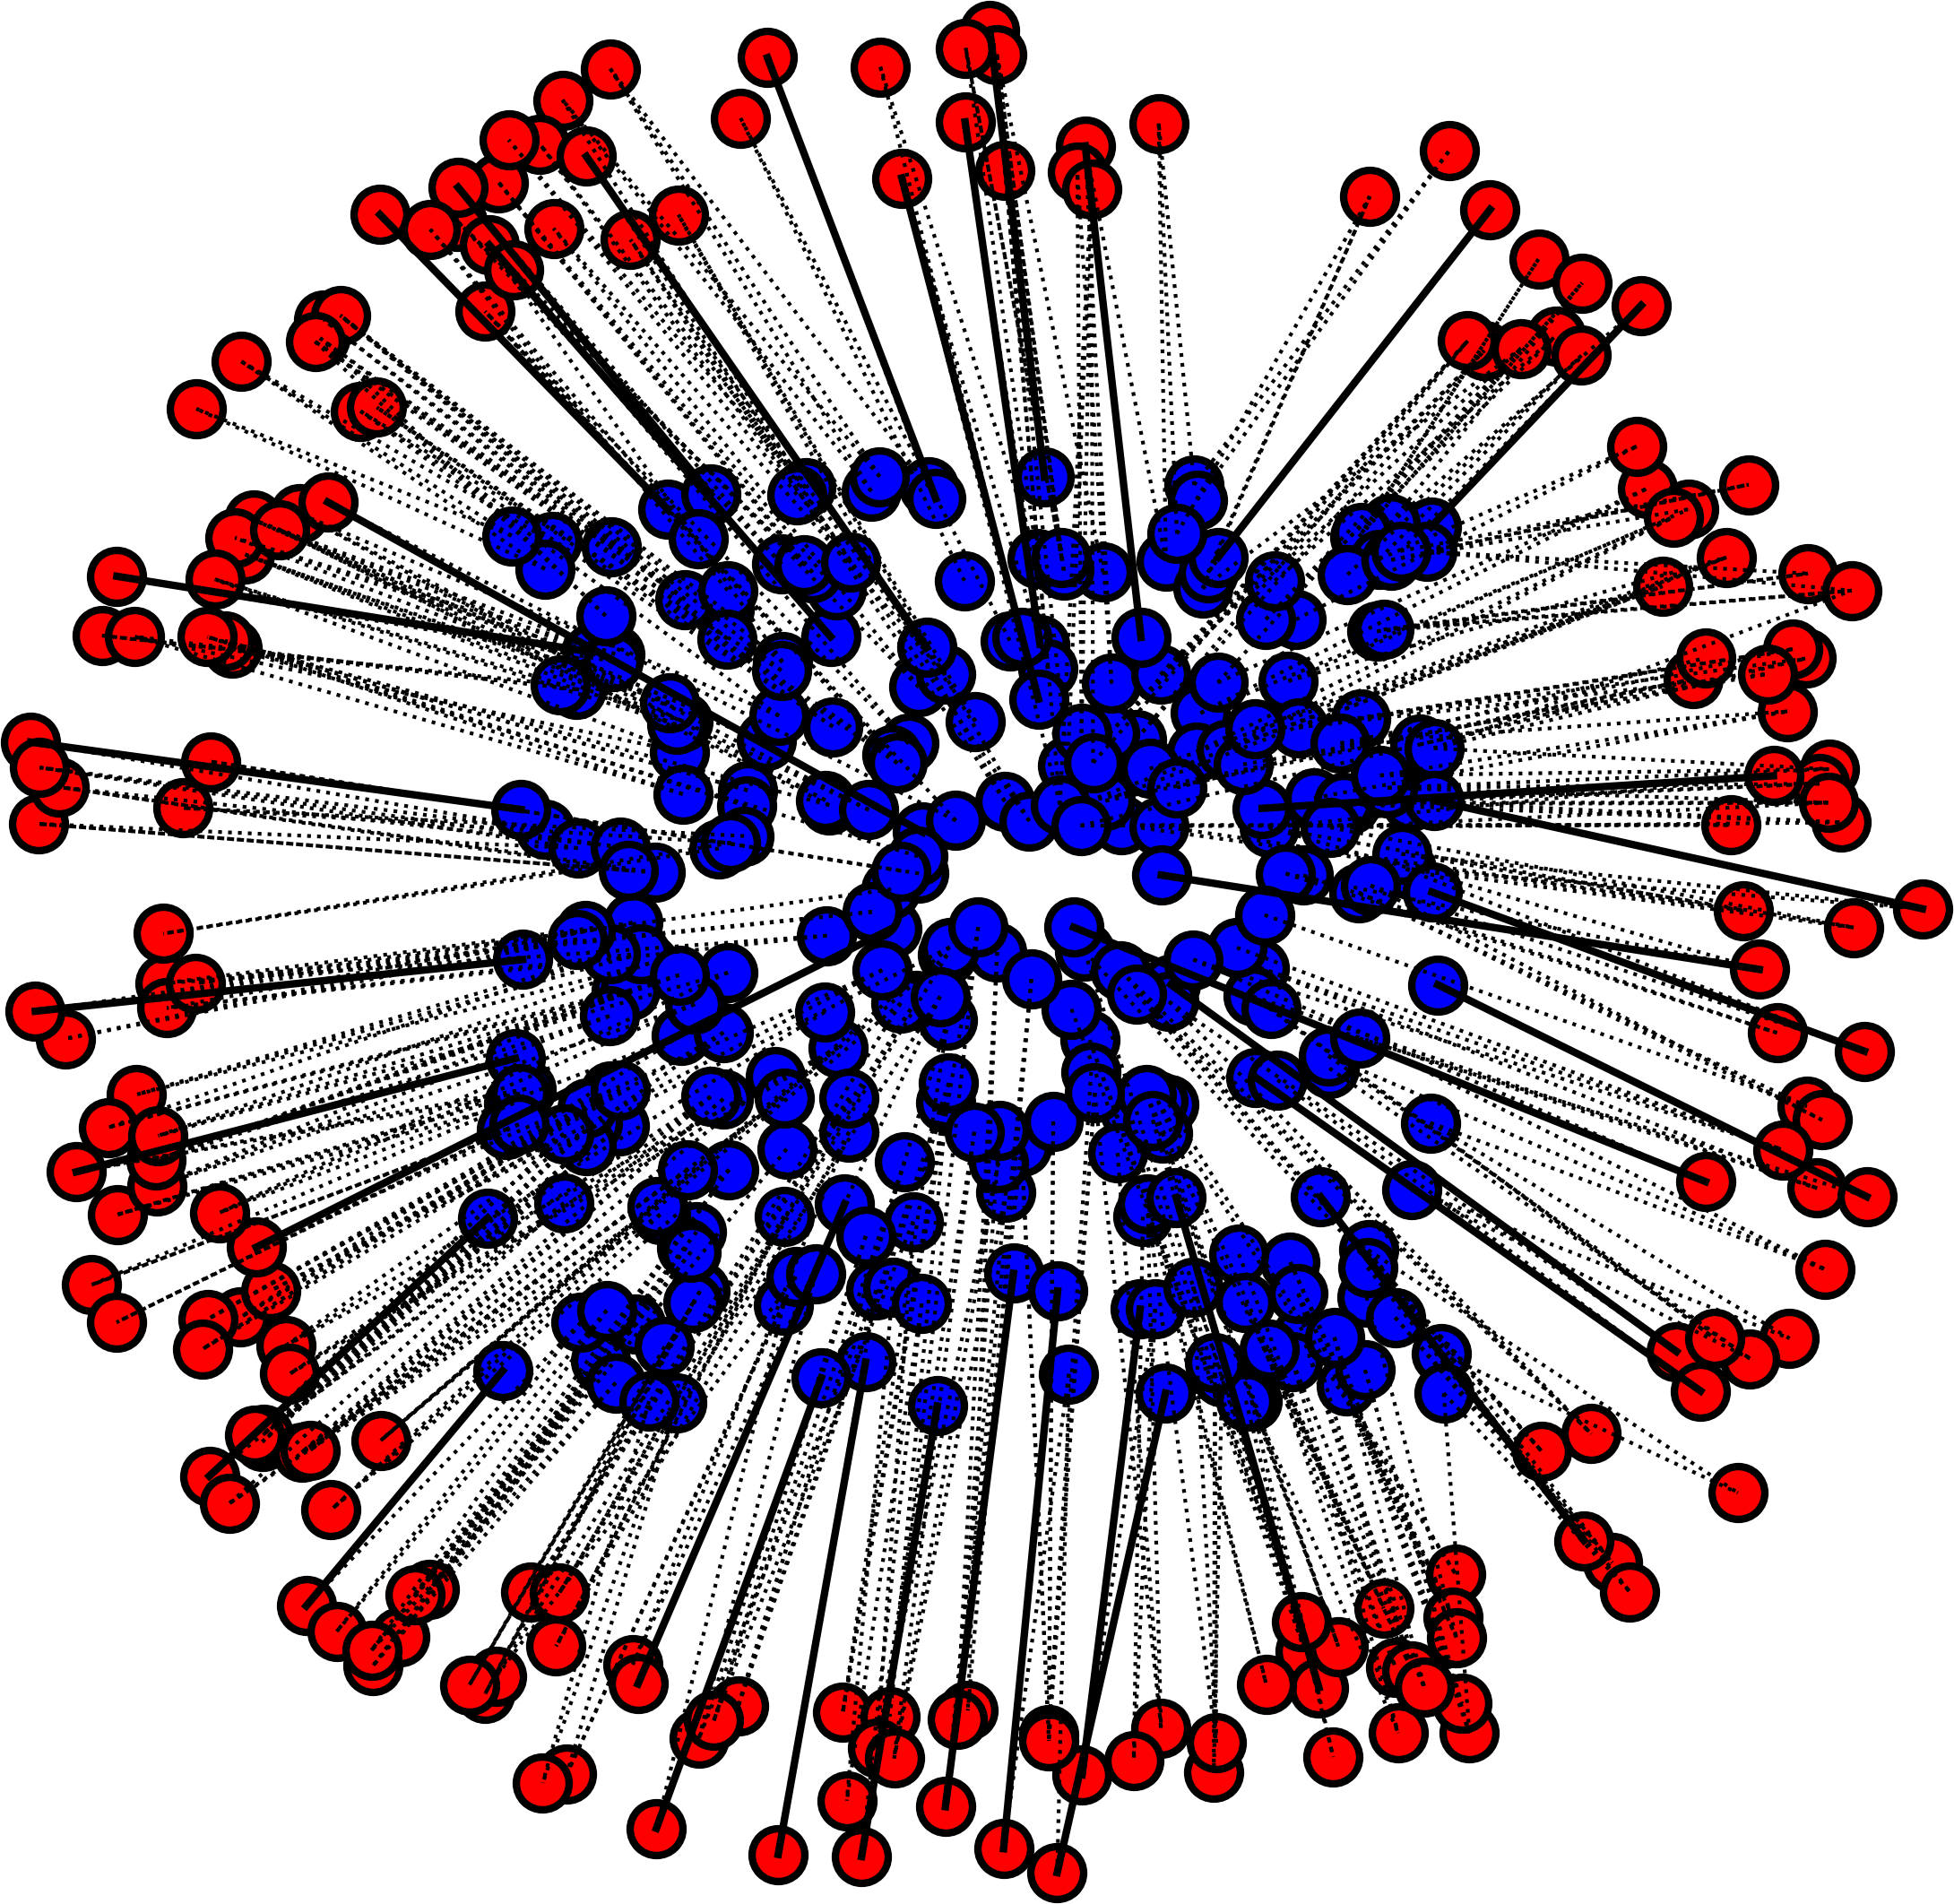
\includegraphics[width=\textwidth]{samples/2/coupling_eps_1e-3.png}
         \caption{$\epsilon=\tenp{-3}$}
     \end{subfigure}
    \caption{Regularized coupling for the same distribution. For low values of $\epsilon$, the coupling is sparse.}
    \label{fig:coupling_eps}
\end{figure}

\FloatBarrier
\subsection{Transport Between Histograms}

We now consider the problem of transporting two discrete measure whose support lies on a grid: $\cb{\frac{k}{n}, k \in \cb{0, \dots, n-1}}$. We first try when the two distributions are Gaussian (fig. \ref{fig:two_histograms}).

\begin{figure}[p]
    \centering
    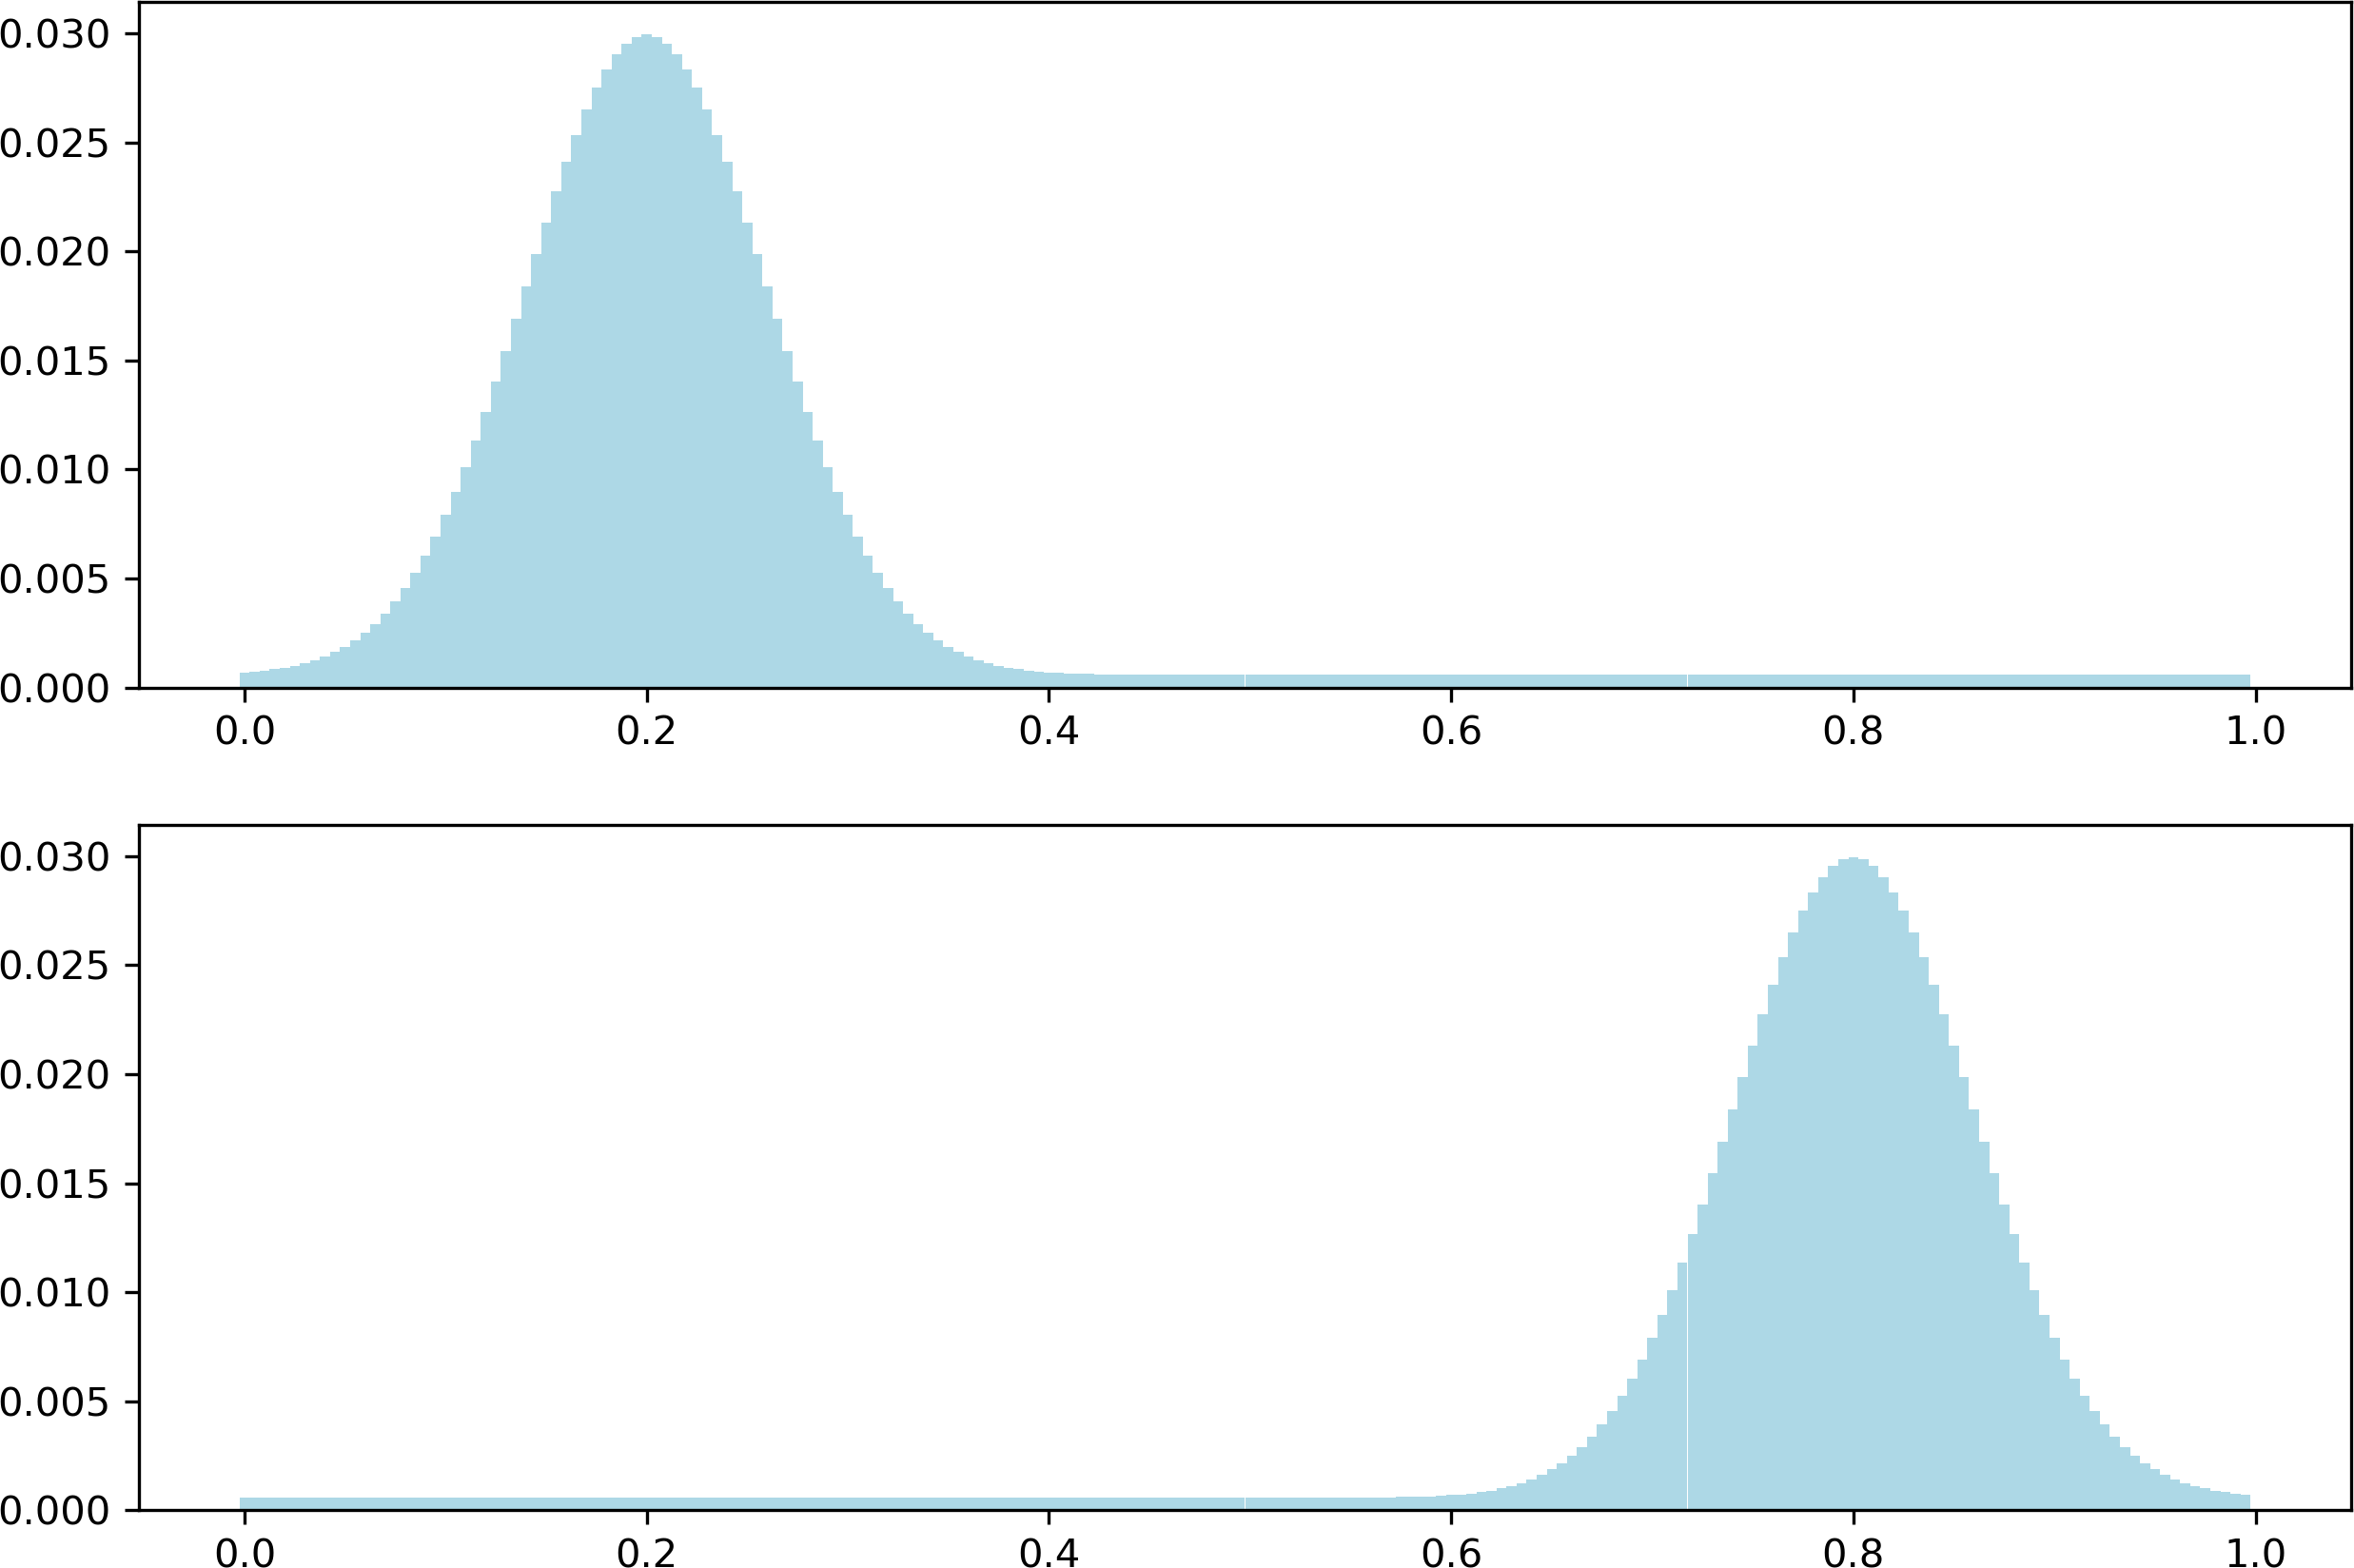
\includegraphics[width=.7\textwidth]{samples/2/two_histograms.png}
    \caption{Two gaussian histograms we will transport.}
    \label{fig:two_histograms}
\end{figure}

Computing the Gibbs kernel yields a Gaussian kernel (fig. \ref{fig:gibbs_kernel}).

\begin{figure}[p]
    \centering
    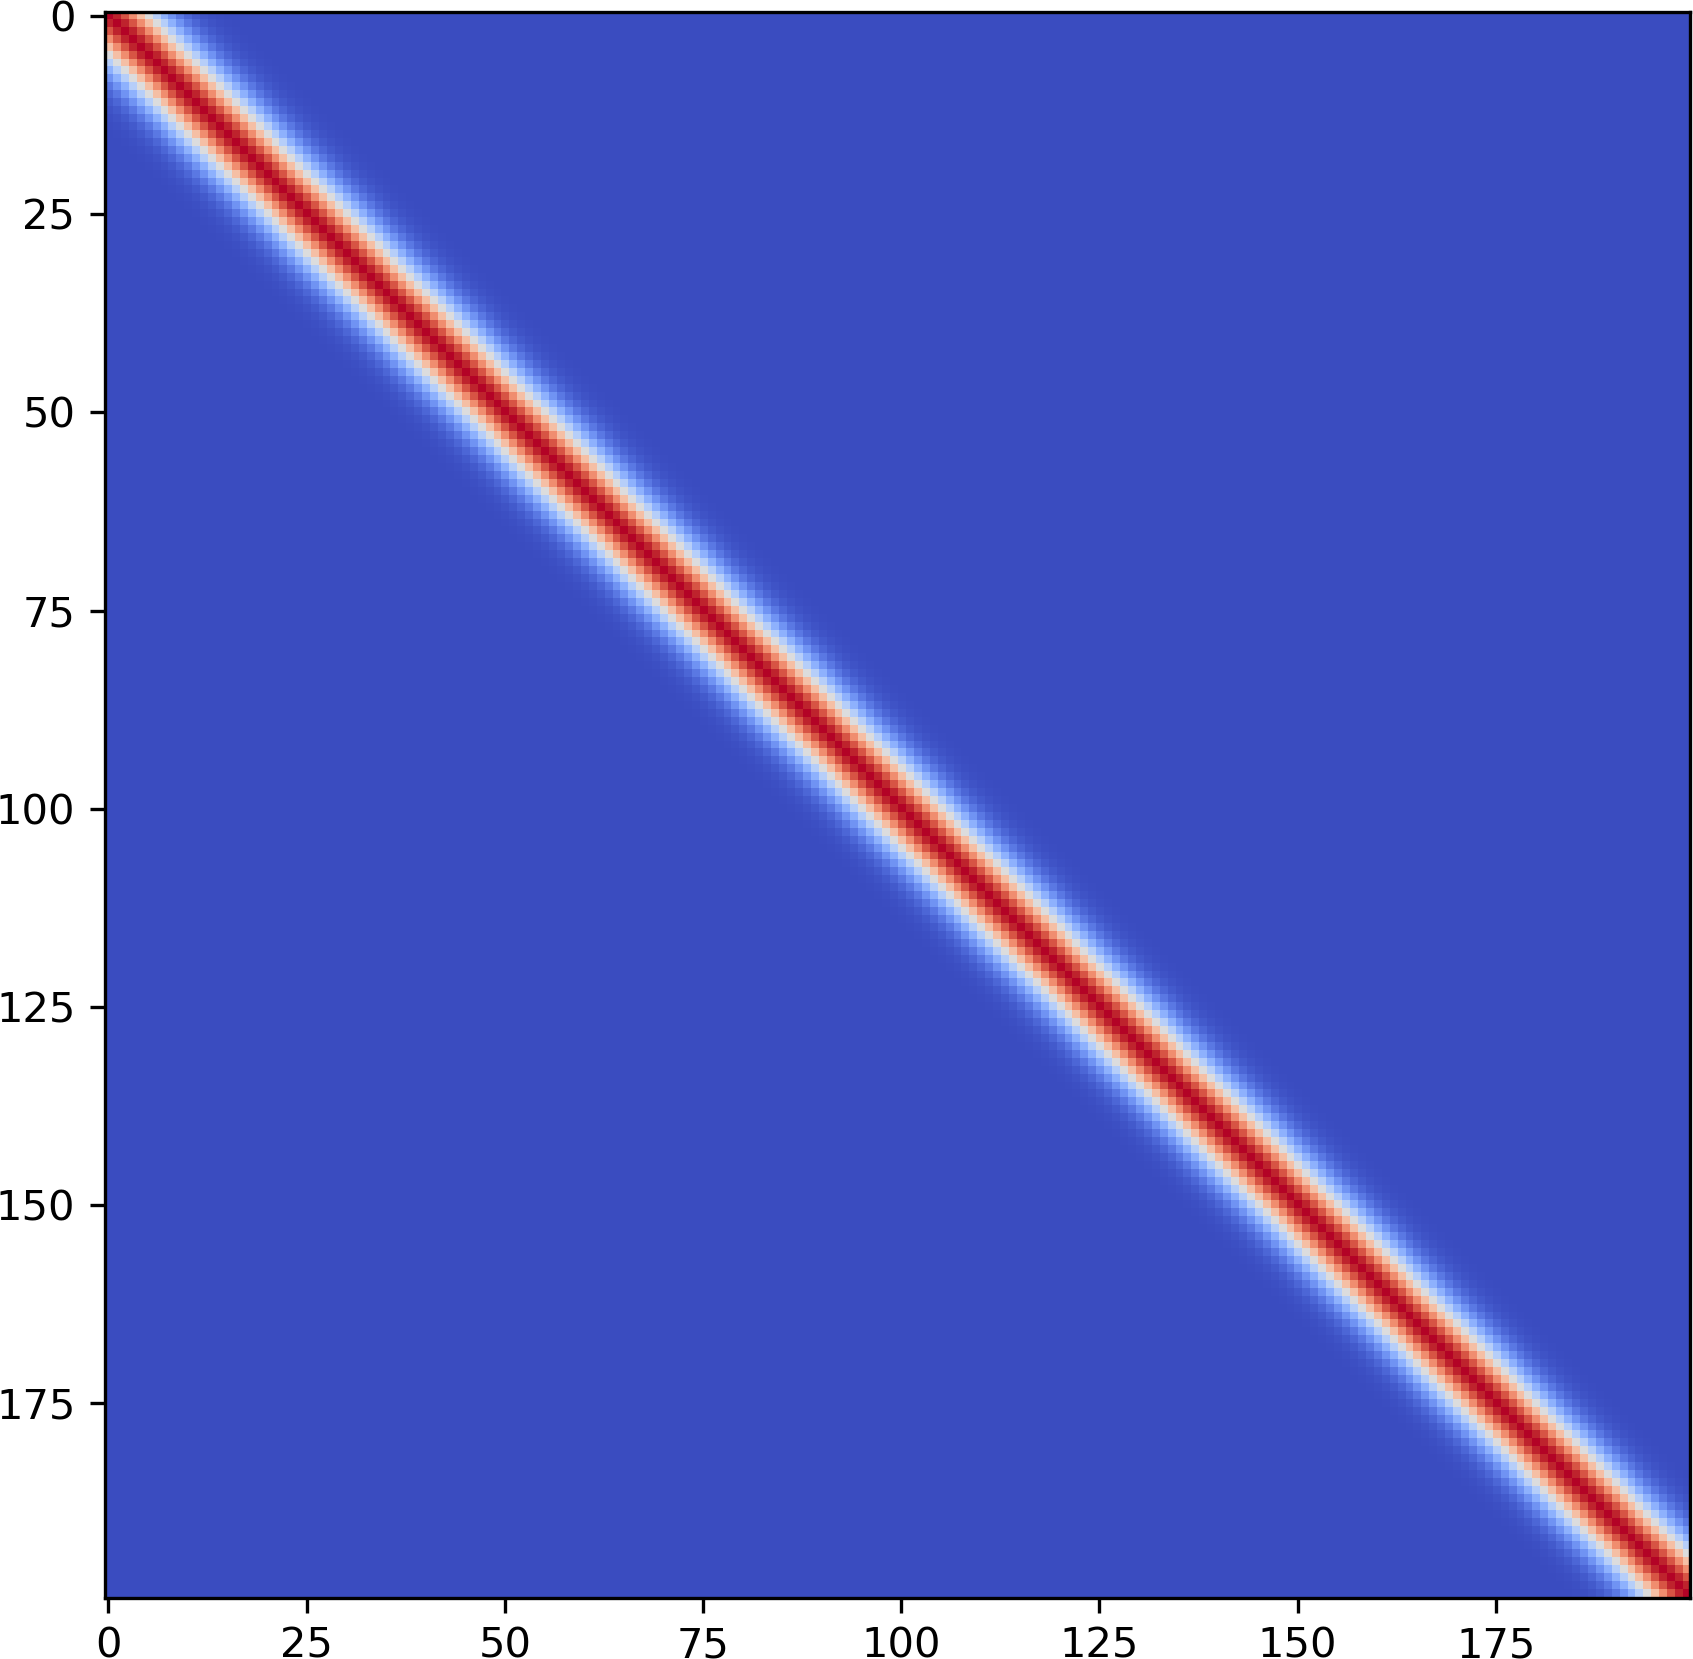
\includegraphics[width=.5\textwidth]{samples/2/gibbs_kernel.png}
    \caption{Computing the Gibbs Kernel of two histograms amounts to computing a Gaussian kernel.}
    \label{fig:gibbs_kernel}
\end{figure}

From there, we can compute the regularized transport plan. The barycentric projection map gives an idea of how the Monge map $T$ looks like (fig. \ref{fig:coupling_histograms}).

\begin{figure}[p]
    \centering
    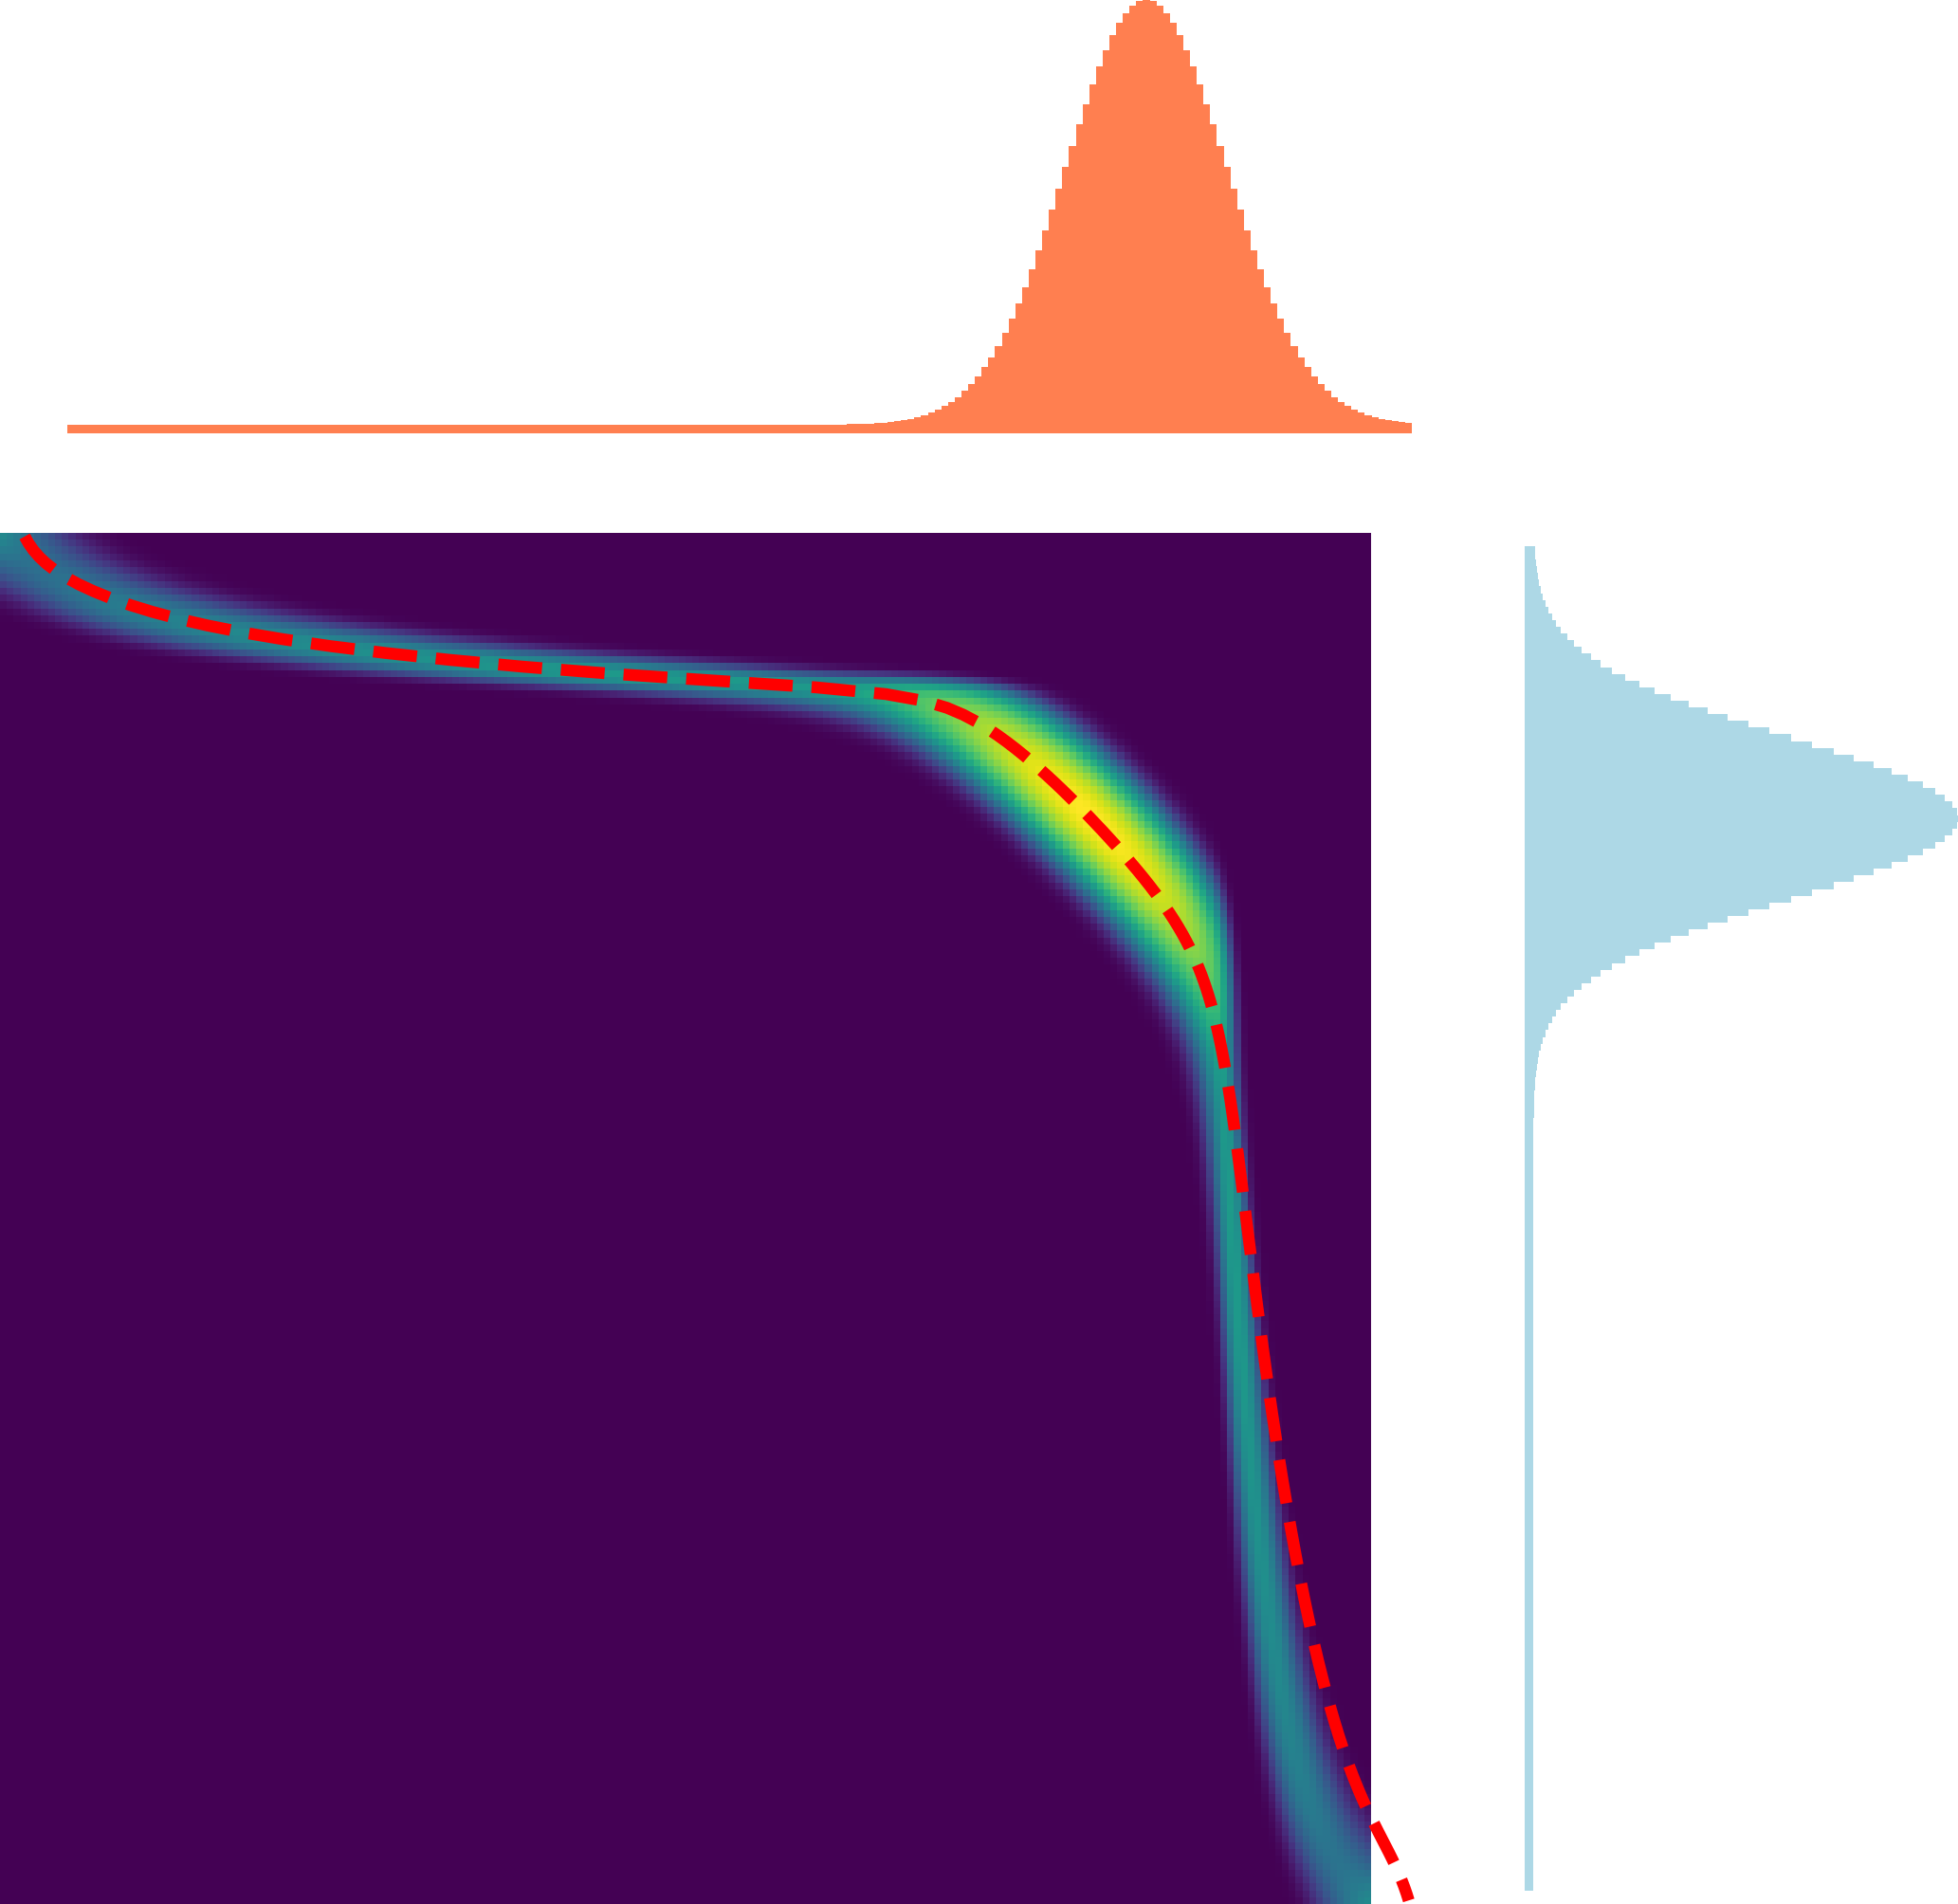
\includegraphics[width=.6\textwidth]{samples/2/coupling_histograms.png}
    \caption{Log of the regularized transport plan. In dots, the barycentric projection gives an approximation of the Monge map.}
    \label{fig:coupling_histograms}
\end{figure}

We can check the goodness of the approximation, function of the regularization parameter $\epsilon$ (fig. \ref{fig:barycentric_maps}).

\begin{figure}[p]
    \centering
    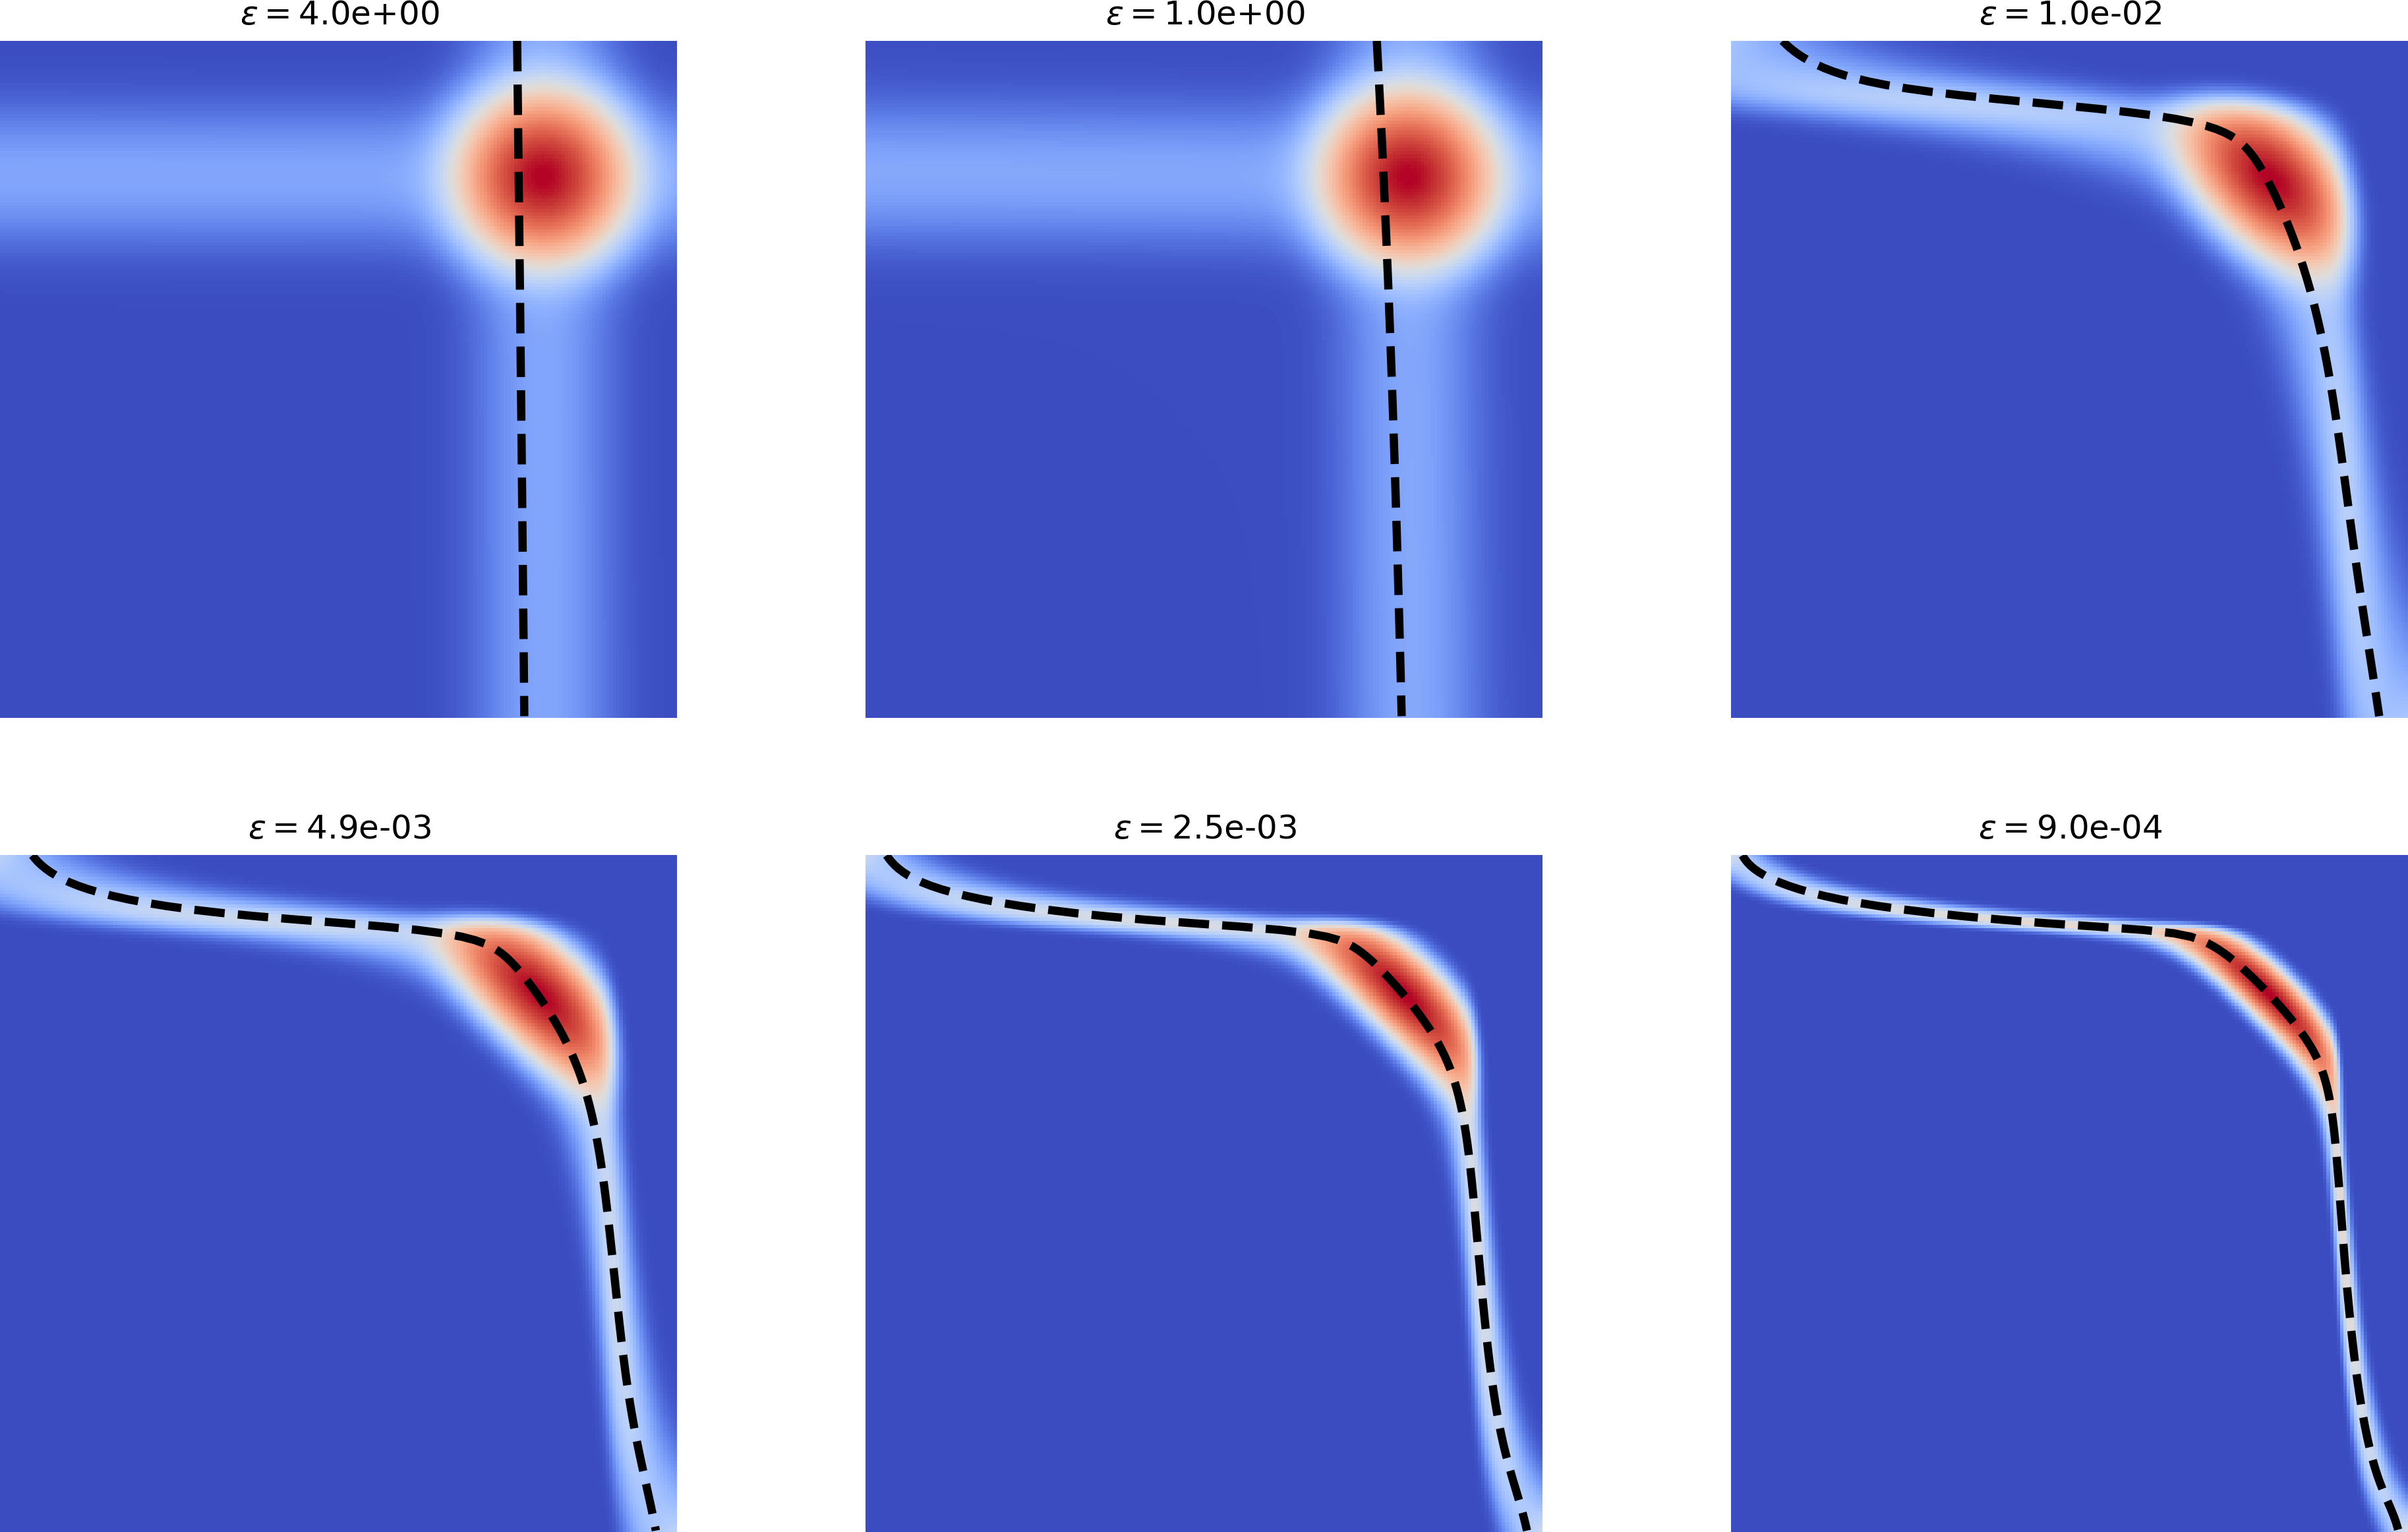
\includegraphics[width=\textwidth]{samples/2/barycentric_maps.png}
    \caption{Barycentric maps for multiple values if $\epsilon$. Notice how diffused the solution is as $\epsilon$ increases. The barycentric map is meaningless for these values.}
    \label{fig:barycentric_maps}
\end{figure}

Finally, taking a look at the transportation of a unimodal distribution to a bimodal distribution gives an interesting hindsight on what happens to the \textit{middle point}. We can suppose that the unregularized transport plan is never attained in this setting. 

\begin{figure}[h]
     \centering
     \begin{subfigure}[b]{0.49\textwidth}
         \centering
         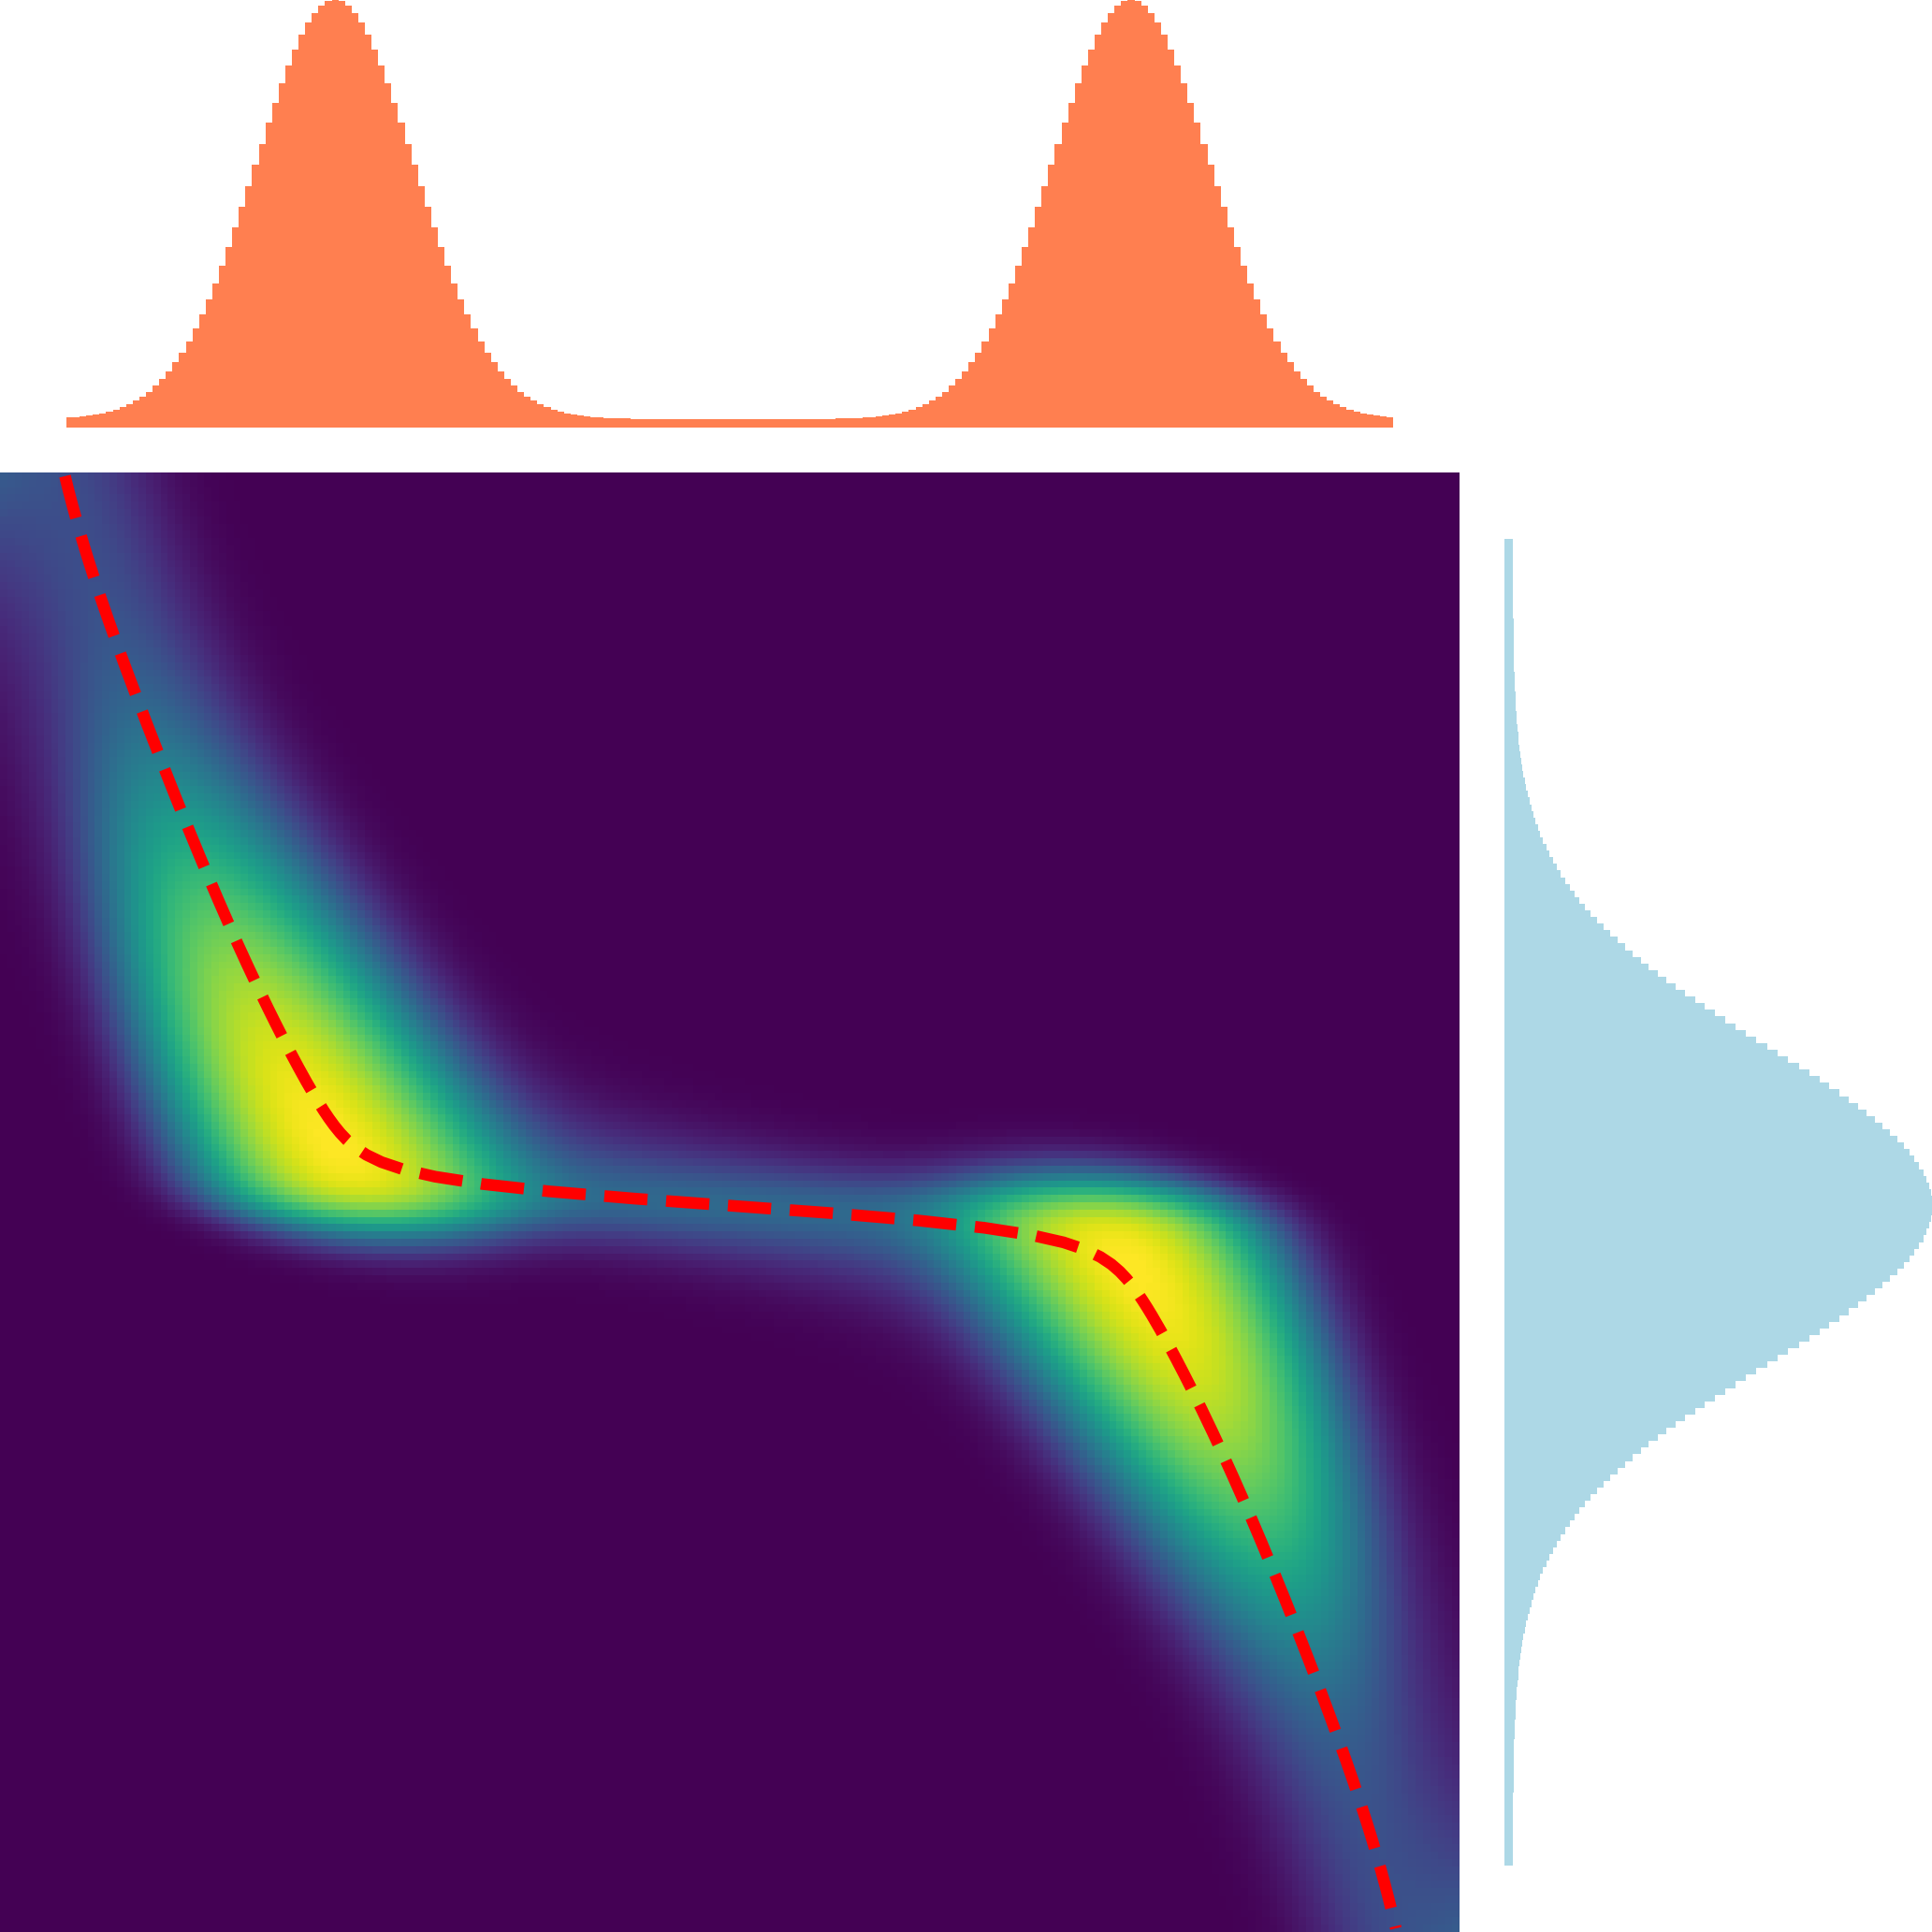
\includegraphics[width=\textwidth]{samples/2/bimodal_transport_histograms_eps_081.png}
         \caption{$\epsilon = 0.09^2$}
     \end{subfigure}
     \hfill
     \begin{subfigure}[b]{0.49\textwidth}
         \centering
         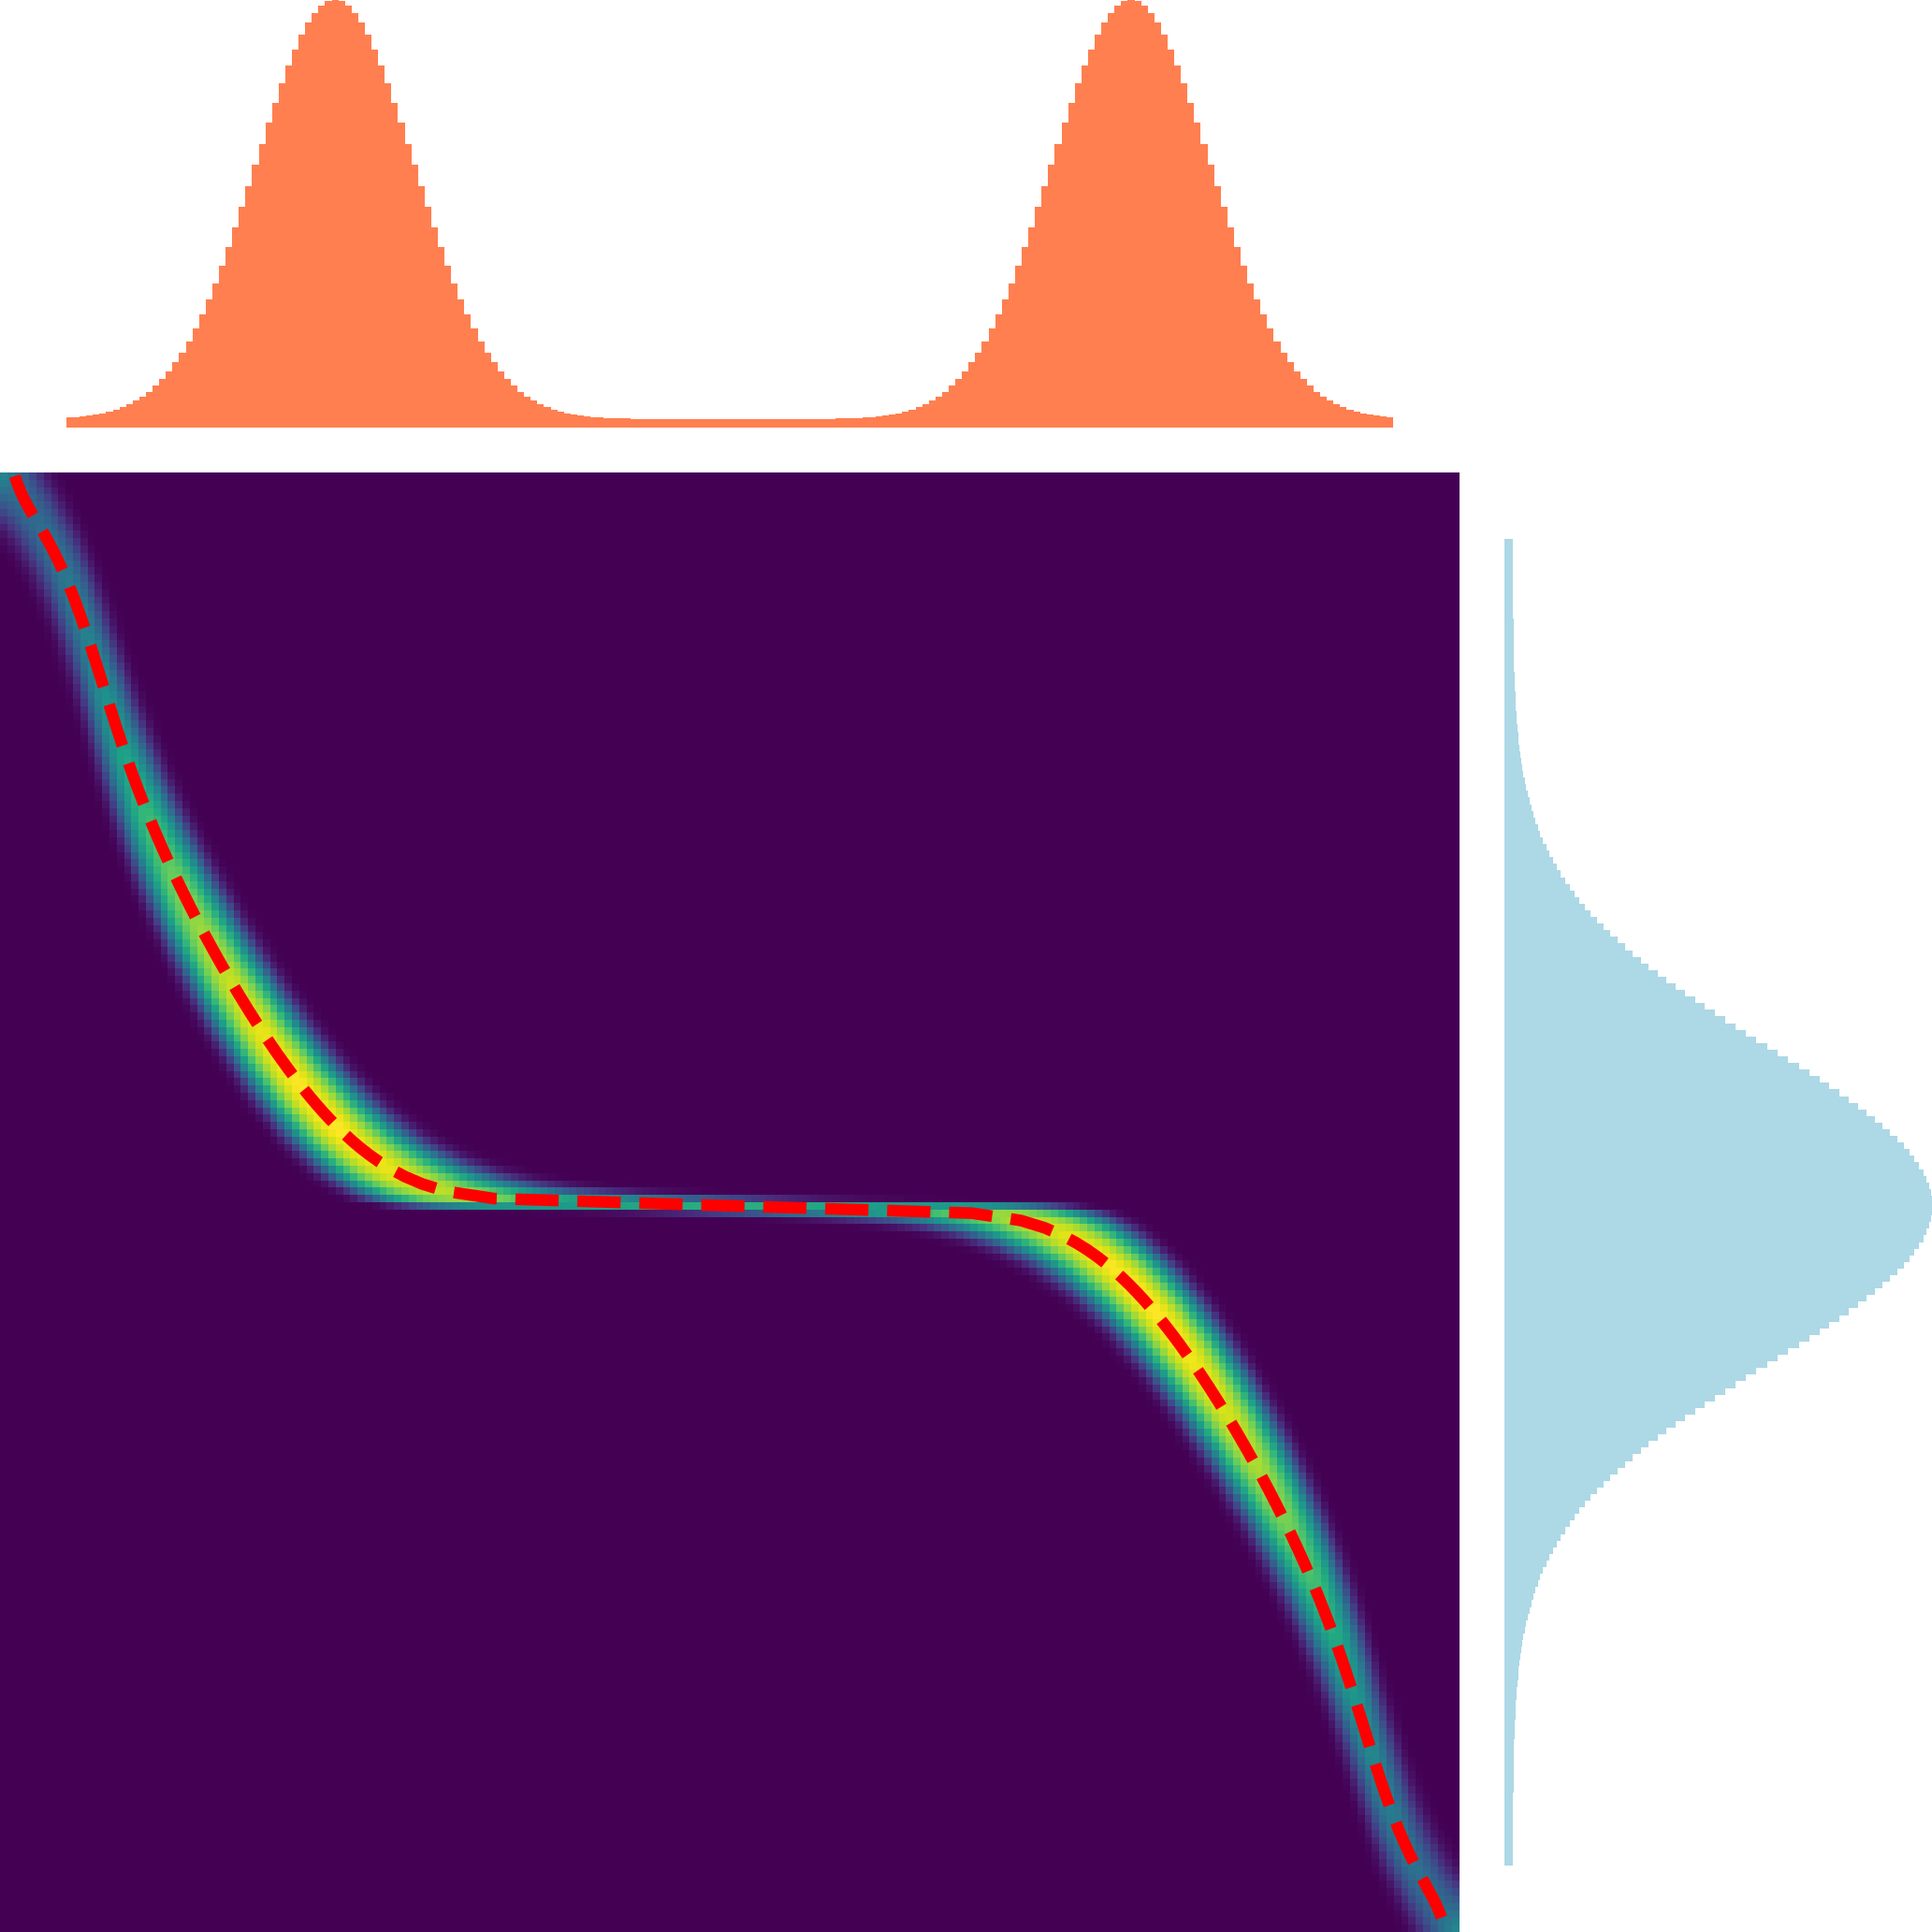
\includegraphics[width=\textwidth]{samples/2/bimodal_transport_histograms_eps_004.png}
         \caption{$\epsilon = 0.02^2$}
     \end{subfigure}
    \caption{Going from a unimodal distribution to a bimodal distribution. As $\epsilon$ goes to $0$ and the coupling converges to the unregularized coupling, we may wonder what happens to the discontinuity in the middle.}
\end{figure}

\subsection{Using GPUs}

It is little to say that I was disappointed by my implementation in PyTorch of Sinkhorn's algorithm. Comparing the execution time for $1000$ iterations on histograms with $N$ elements for a constant regularization $\epsilon = 0.06^2$, I obtained the graph shown fig. \ref{fig:gpu_vs_cpu}.

I am not a specialist of PyTorch, so my code may contain errors. Of course, I expected that for small values of $N$, the CPU would get ahead: building the computation graph implies some overhead. Yet, I thought that for large values, the GPU would completely destroy the CPU's performance. The code was ran on Google Colab. For this execution, the remote machine had an \texttt{Intel(R) Xeon(R) CPU @ 2.00GHz} for CPU and a \texttt{Tesla P100-PCIE} as a GPU. So that can't explain either why the performance are this low. 

\begin{figure}[p]
    \centering
    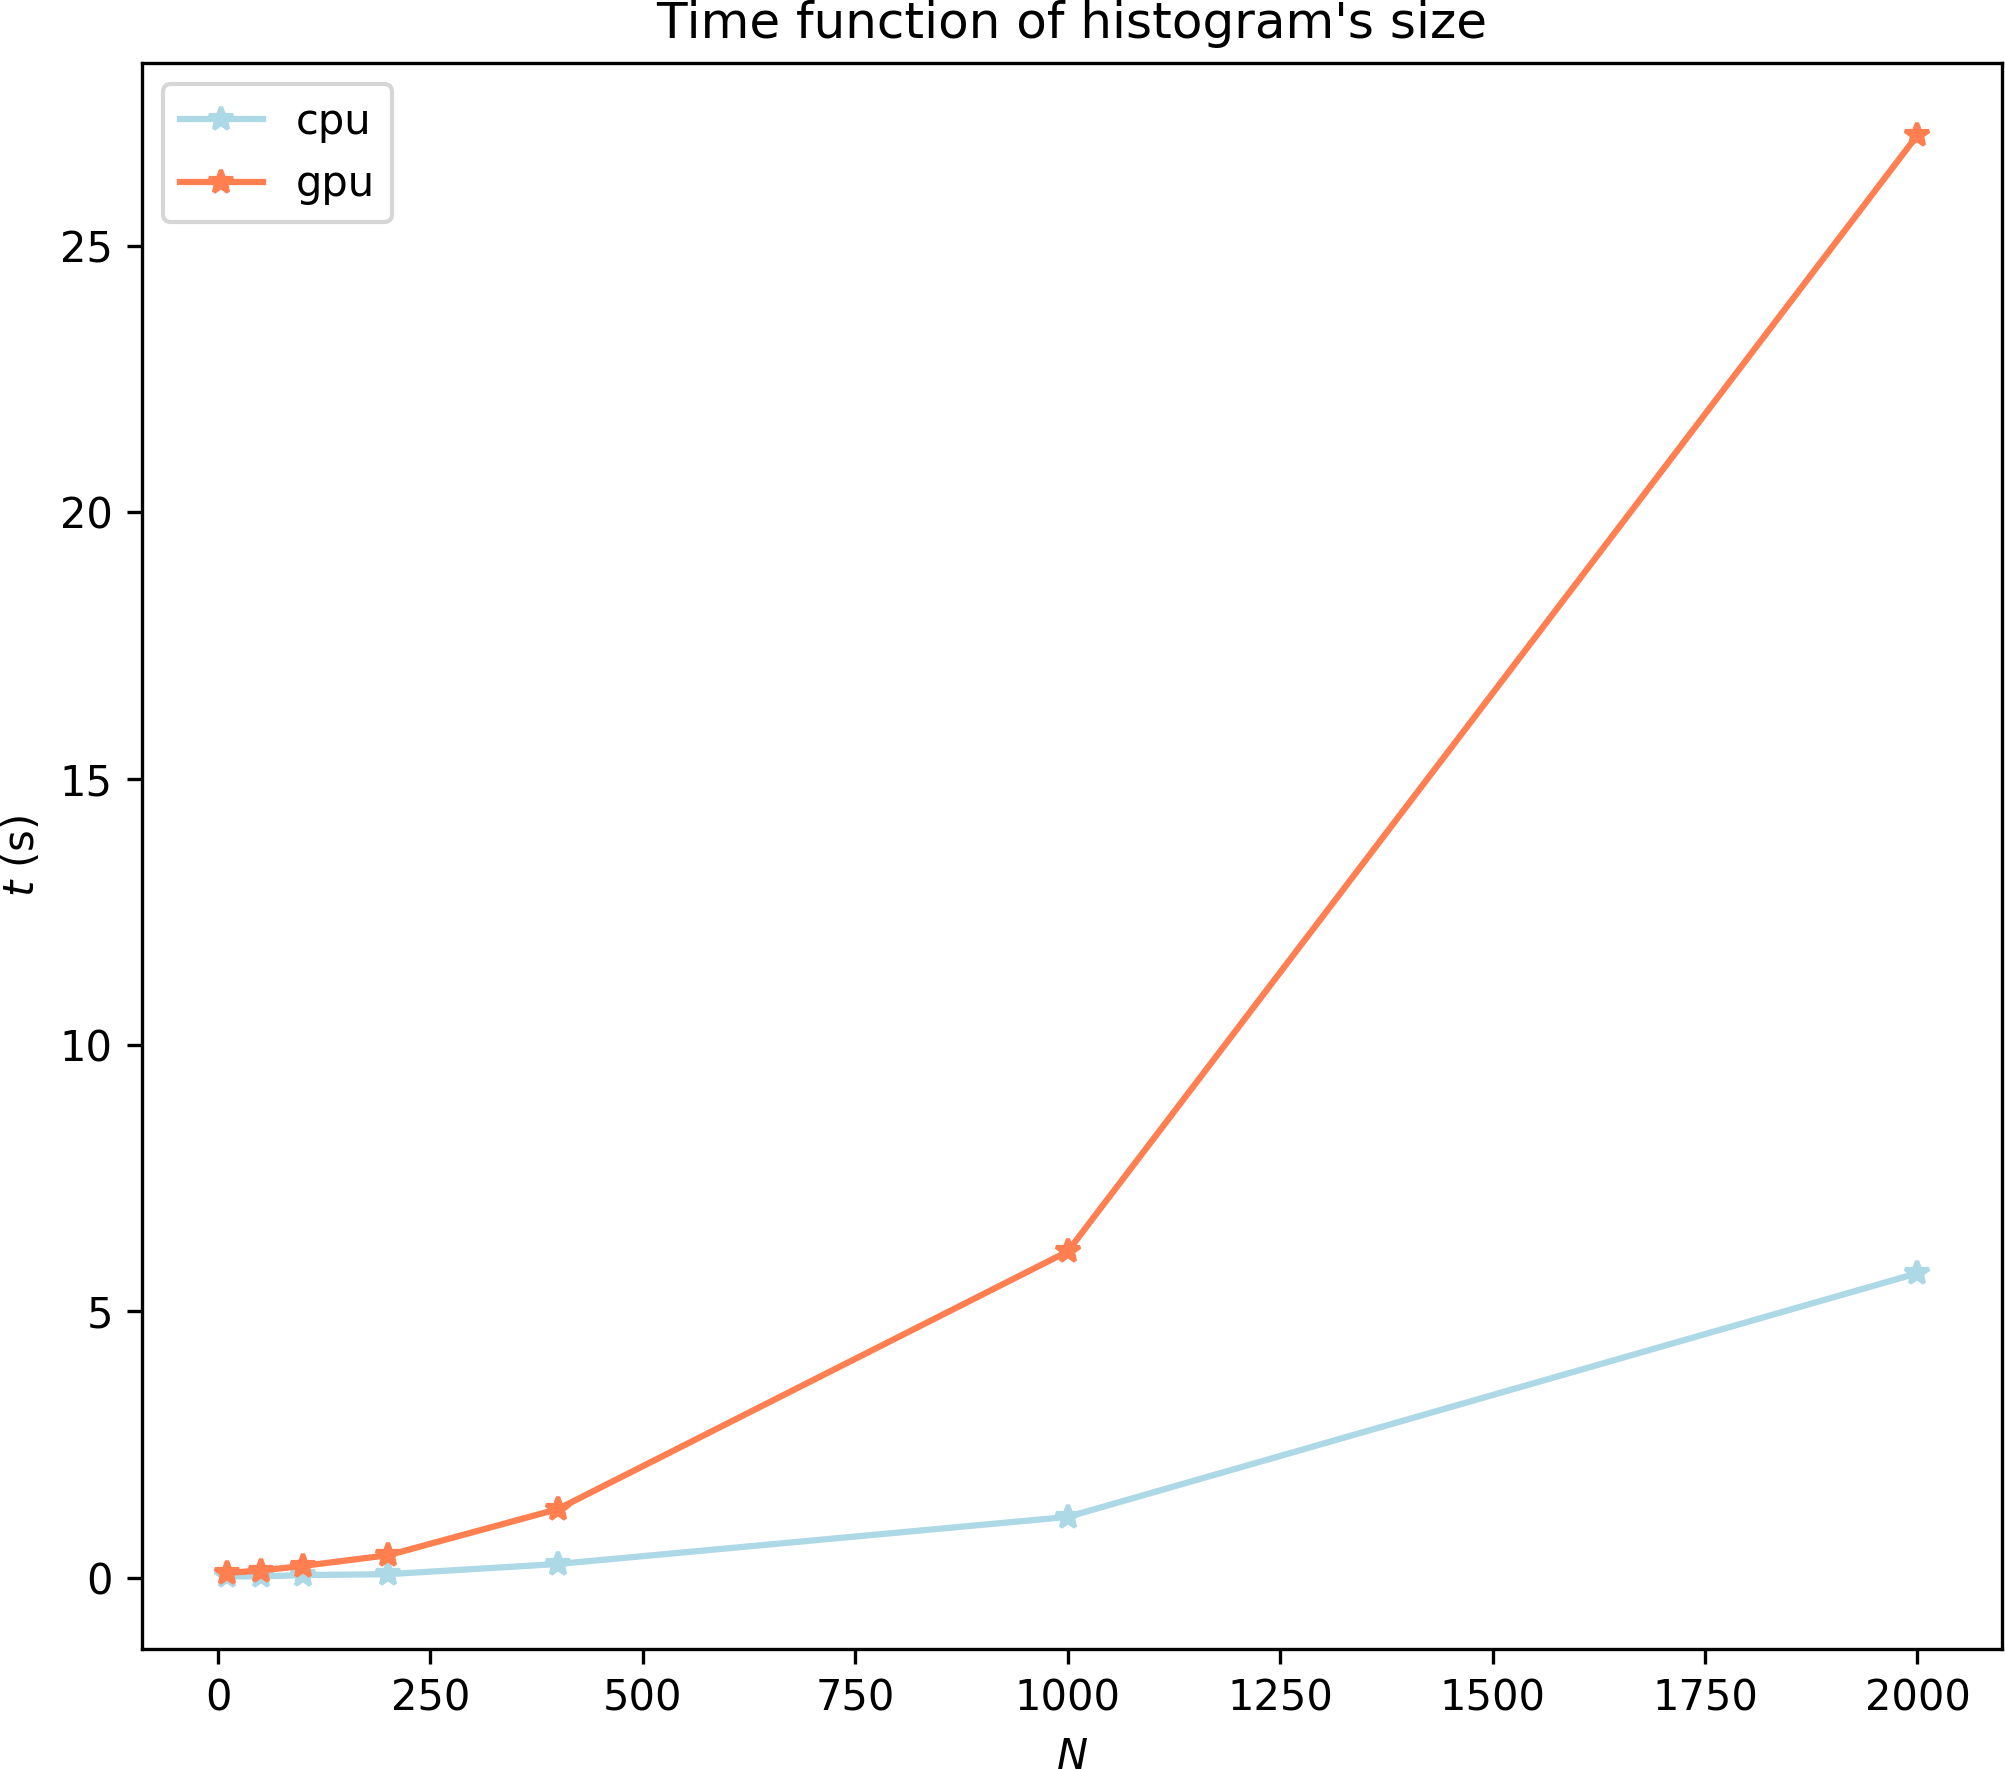
\includegraphics[width=.7\textwidth]{samples/2/gpu_vs_cpu.png}
    \caption{Comparing GPU vs. CPU execution times. To my utter disbelief, the red curve is in fact corresponding to the GPU performance.}
    \label{fig:gpu_vs_cpu}
\end{figure}

\FloatBarrier
\subsection{Wasserstein barycenters}

Here, I tried to see to what extent the Wasserstein barycenter could be used for image registration. Basically, let's say we have a set of brain scans. To compute statistics over this set, and give a meaning to mean, standard deviation, cluster or whatever, we need to specify a \textit{distance} between our images. Optimal transport is a solution to that problem. 

Concerning Wasserstein barycenters, I wondered if the barycenter of multiple brain scans could be used as a \textbf{mean} accross all our samples. Such mean is referred to as \textbf{atlas} in the corresponding literature. 

So here was my question; can the Wasserstein barycenter of multiple brain scans be a relevant atlas? 

\subsubsection{Data}

I did not have at my disposal fresh and real brain scans. So I generated \textit{phantom brains}, which simply consist of ellipses at several specific points on the image. They correspond to a basic saggital cut of the brain. To denote the \textbf{variability} across individual, I dilated, translated, rotated each of these ellipses randomly.

The basis phantom is shown in fig. \ref{fig:phantom_brains}, along with samples from it.

\begin{figure}[h]
    \centering
    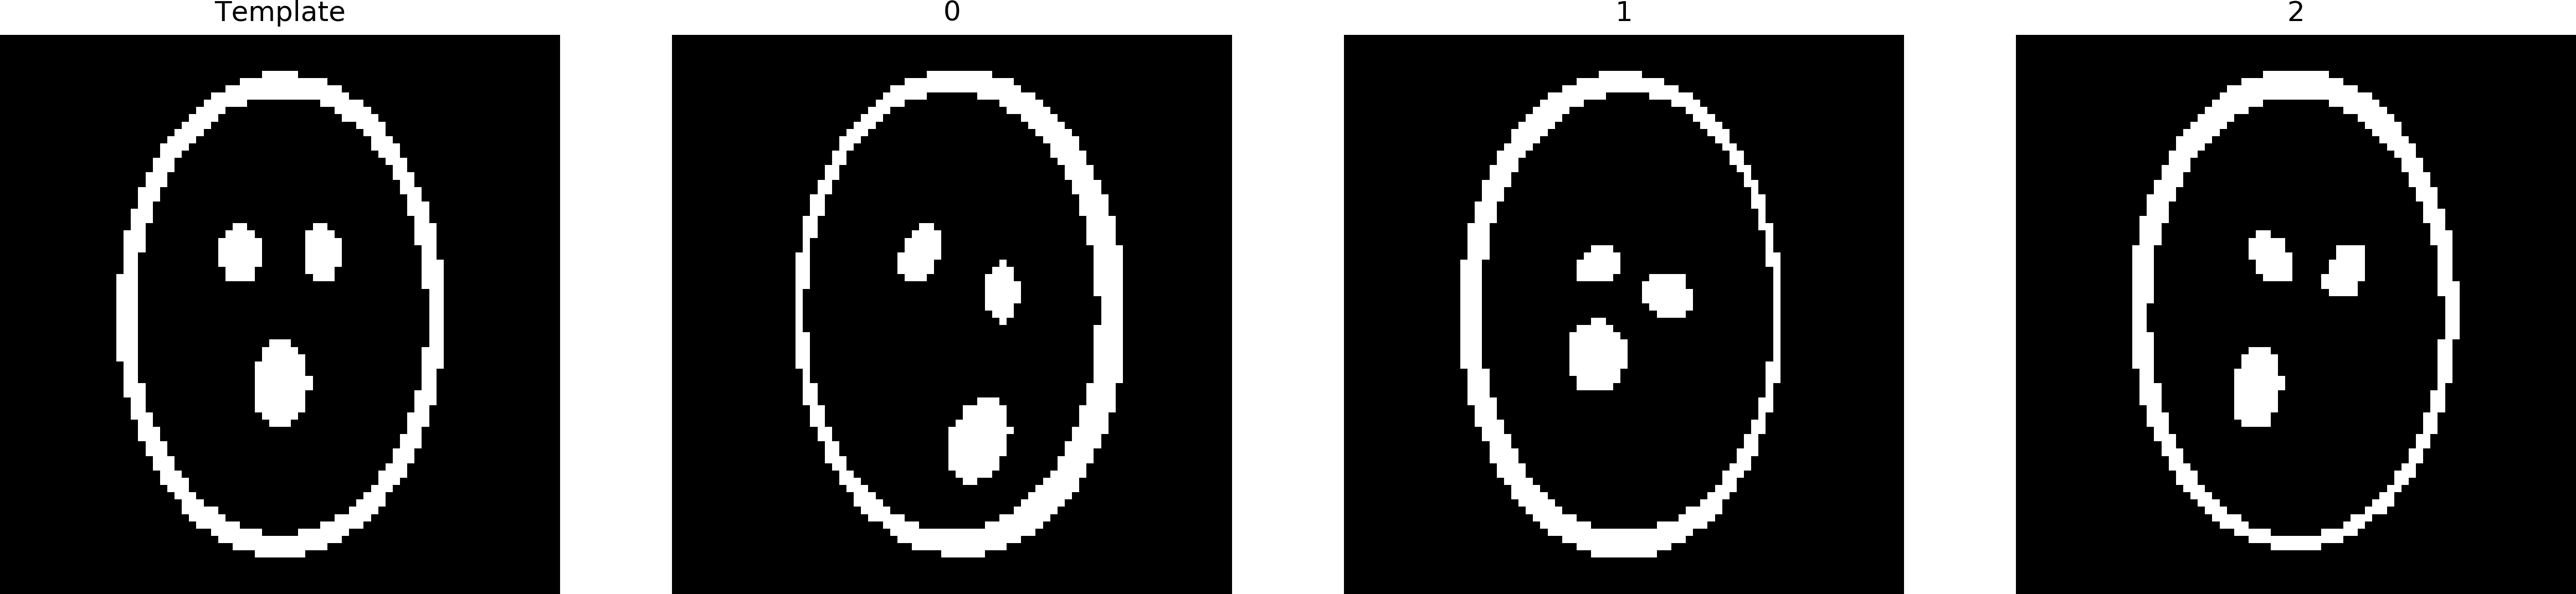
\includegraphics[width=.8\textwidth]{samples/2/phantom_brains.png}
    \caption{The template (left) and three sampled phantoms.}
    \label{fig:phantom_brains}
\end{figure}

In a second attempt, I chose simpler shapes as input. Those are disks whose center lies on a circle, center in the middle of the image. Samples are shown on fig. \ref{fig:circles}.

\begin{figure}[h]
    \centering
    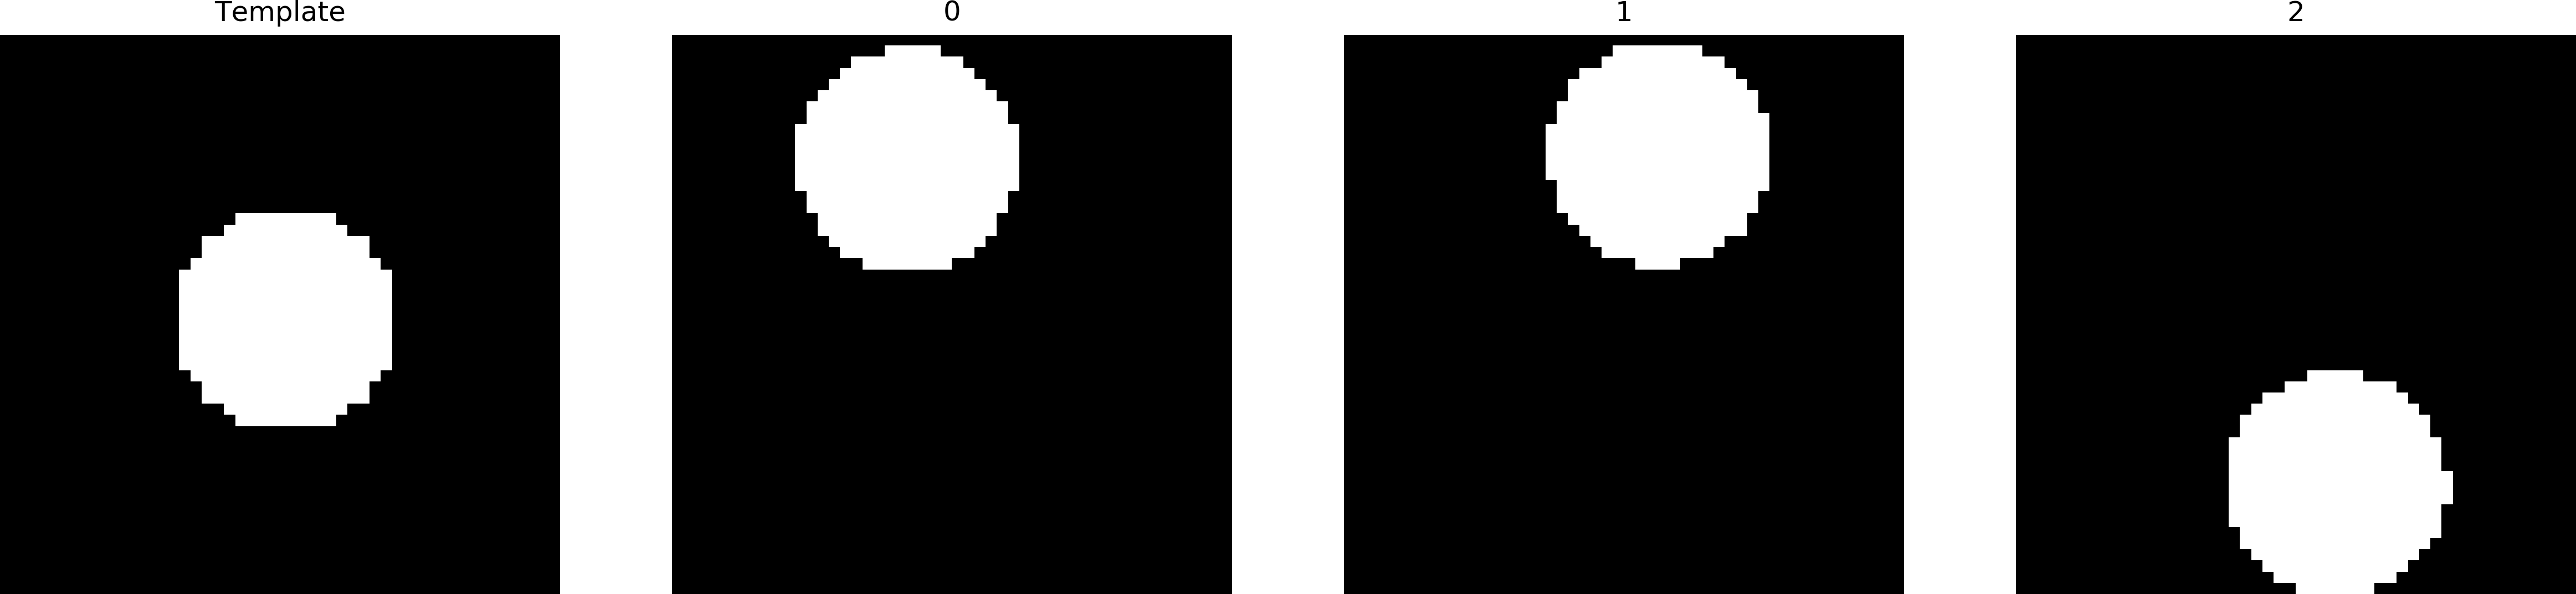
\includegraphics[width=.8\textwidth]{samples/2/some_circles.png}
    \caption{The template (left) and three sampled circles.}
    \label{fig:circles}
\end{figure}

\FloatBarrier
\subsubsection{Result}

I struggled quite a bit to get this part right. My first assumption was: "the more samples you have, the better is the barycenter". In fact, the number of samples is far from being the bottleneck here. Rather, it's the \textbf{$\mathbf{\epsilon}$ parameter of the entropy} which is the real issue. Indeed, we quickly have enough samples to have a stable barycenter. However, we need to lower $\epsilon$ a lot to get a precise result.

More precisely: 
\begin{itemize}
    \item Refer to fig. \ref{fig:all_brains} to get an overview of the evolution of the quality of the barycenter for various number of phantom brain samples and entropic parameter $\epsilon$. Refer to fig. \ref{fig:all_circles} for the same picture with the circles dataset. 
    \item Refer to fig. \ref{fig:l2_loss_brain} and \ref{fig:l2_loss_circle} for the evolution of the loss, function of $\epsilon$ and the number of samples. You might notice that the $L_2$ loss was a poor choice\footnote{\label{my_error}In fact, I truly lacked insights here: I searched for a while a good loss, trying $L_1$, $L_2$ or a "dice-score" loss. But it's precisely the purpose of OT to leverage a distance between points to yield a distance between distributions! My bad.}.
    \item Chronologically, I started with the phantom brains data set, with a fixed $\epsilon=0.01$. I tried computing the barycenter with \textit{a lot} of samples (up to a 1000), until I realized my error: we are not computing the optimal barycenter, but merely an entropic regularization of it.
\end{itemize}

\begin{figure}[p]
    \centering
    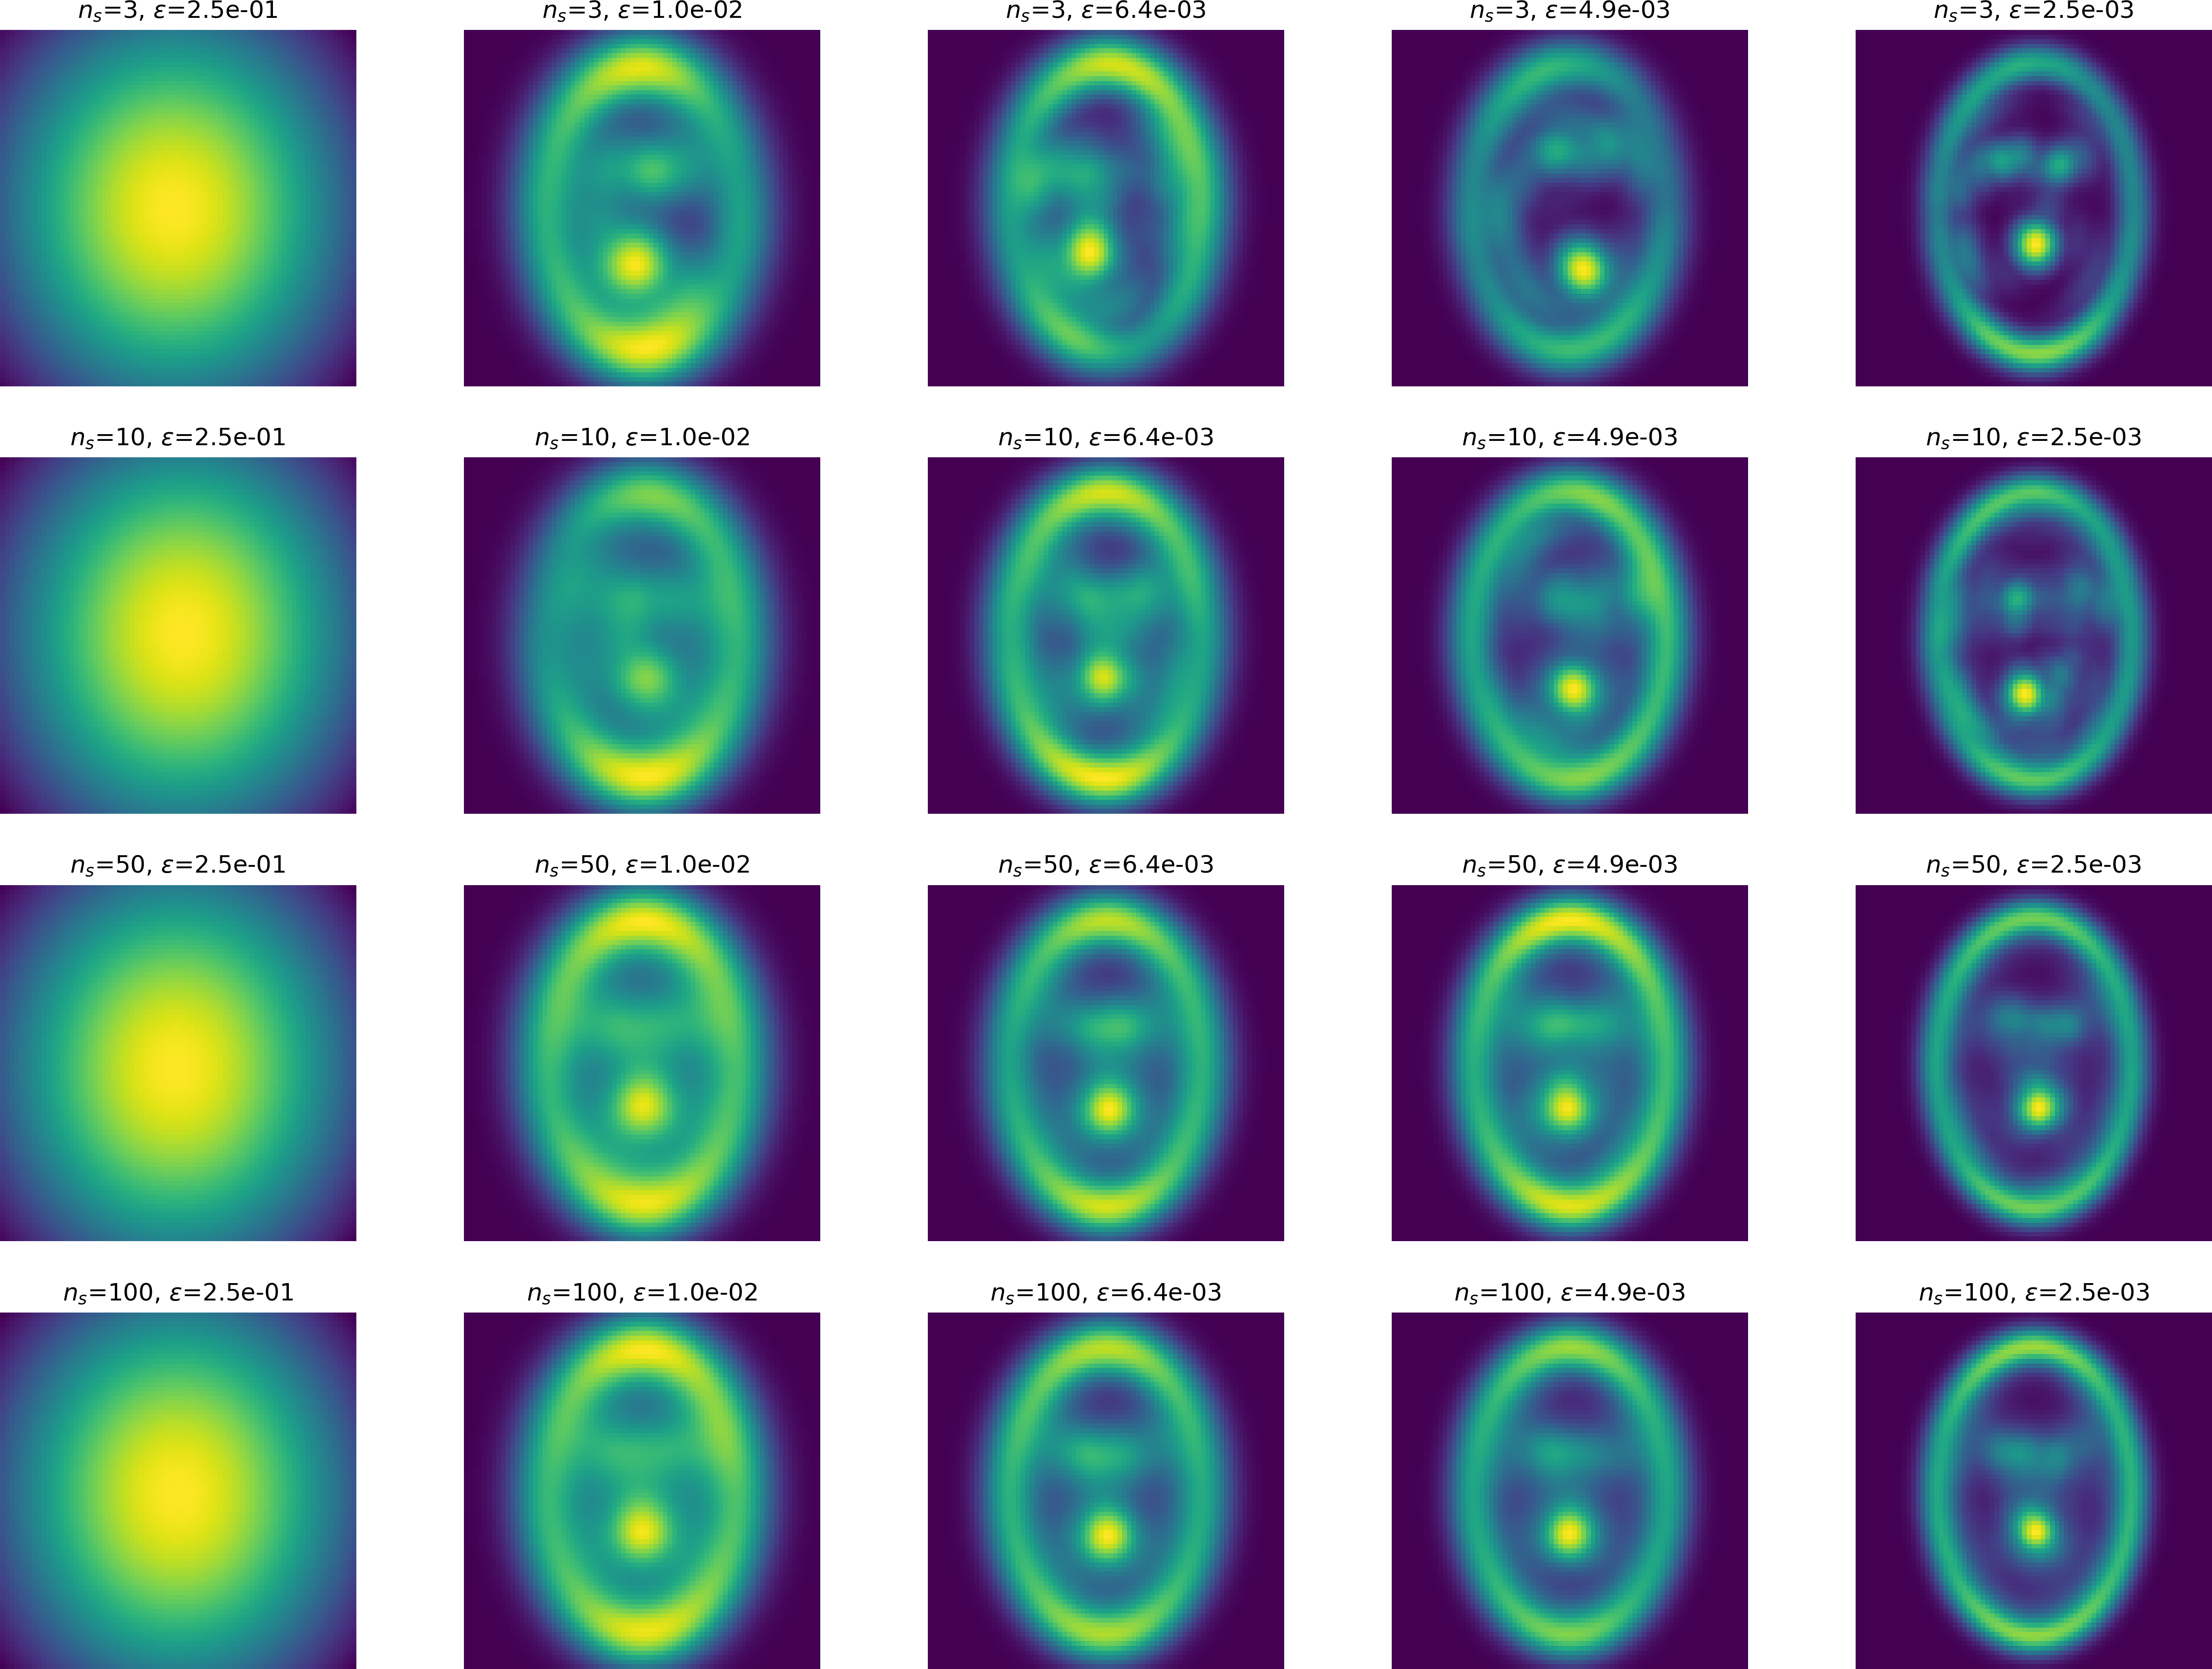
\includegraphics[width=.9\textwidth]{samples/2/all_brains.png}
    \caption{Barycenter of multiple sampled brains. On \textbf{rows} are varying number of samples $n_s$, ranging from $3$ to $100$. On columns are varying values of $\epsilon$, ranging from $0.5^2$ to $0.05^2$. Notice how quickly having more samples becomes irrelevant.}
    \label{fig:all_brains}
\end{figure}

\begin{figure}[p]
    \centering
    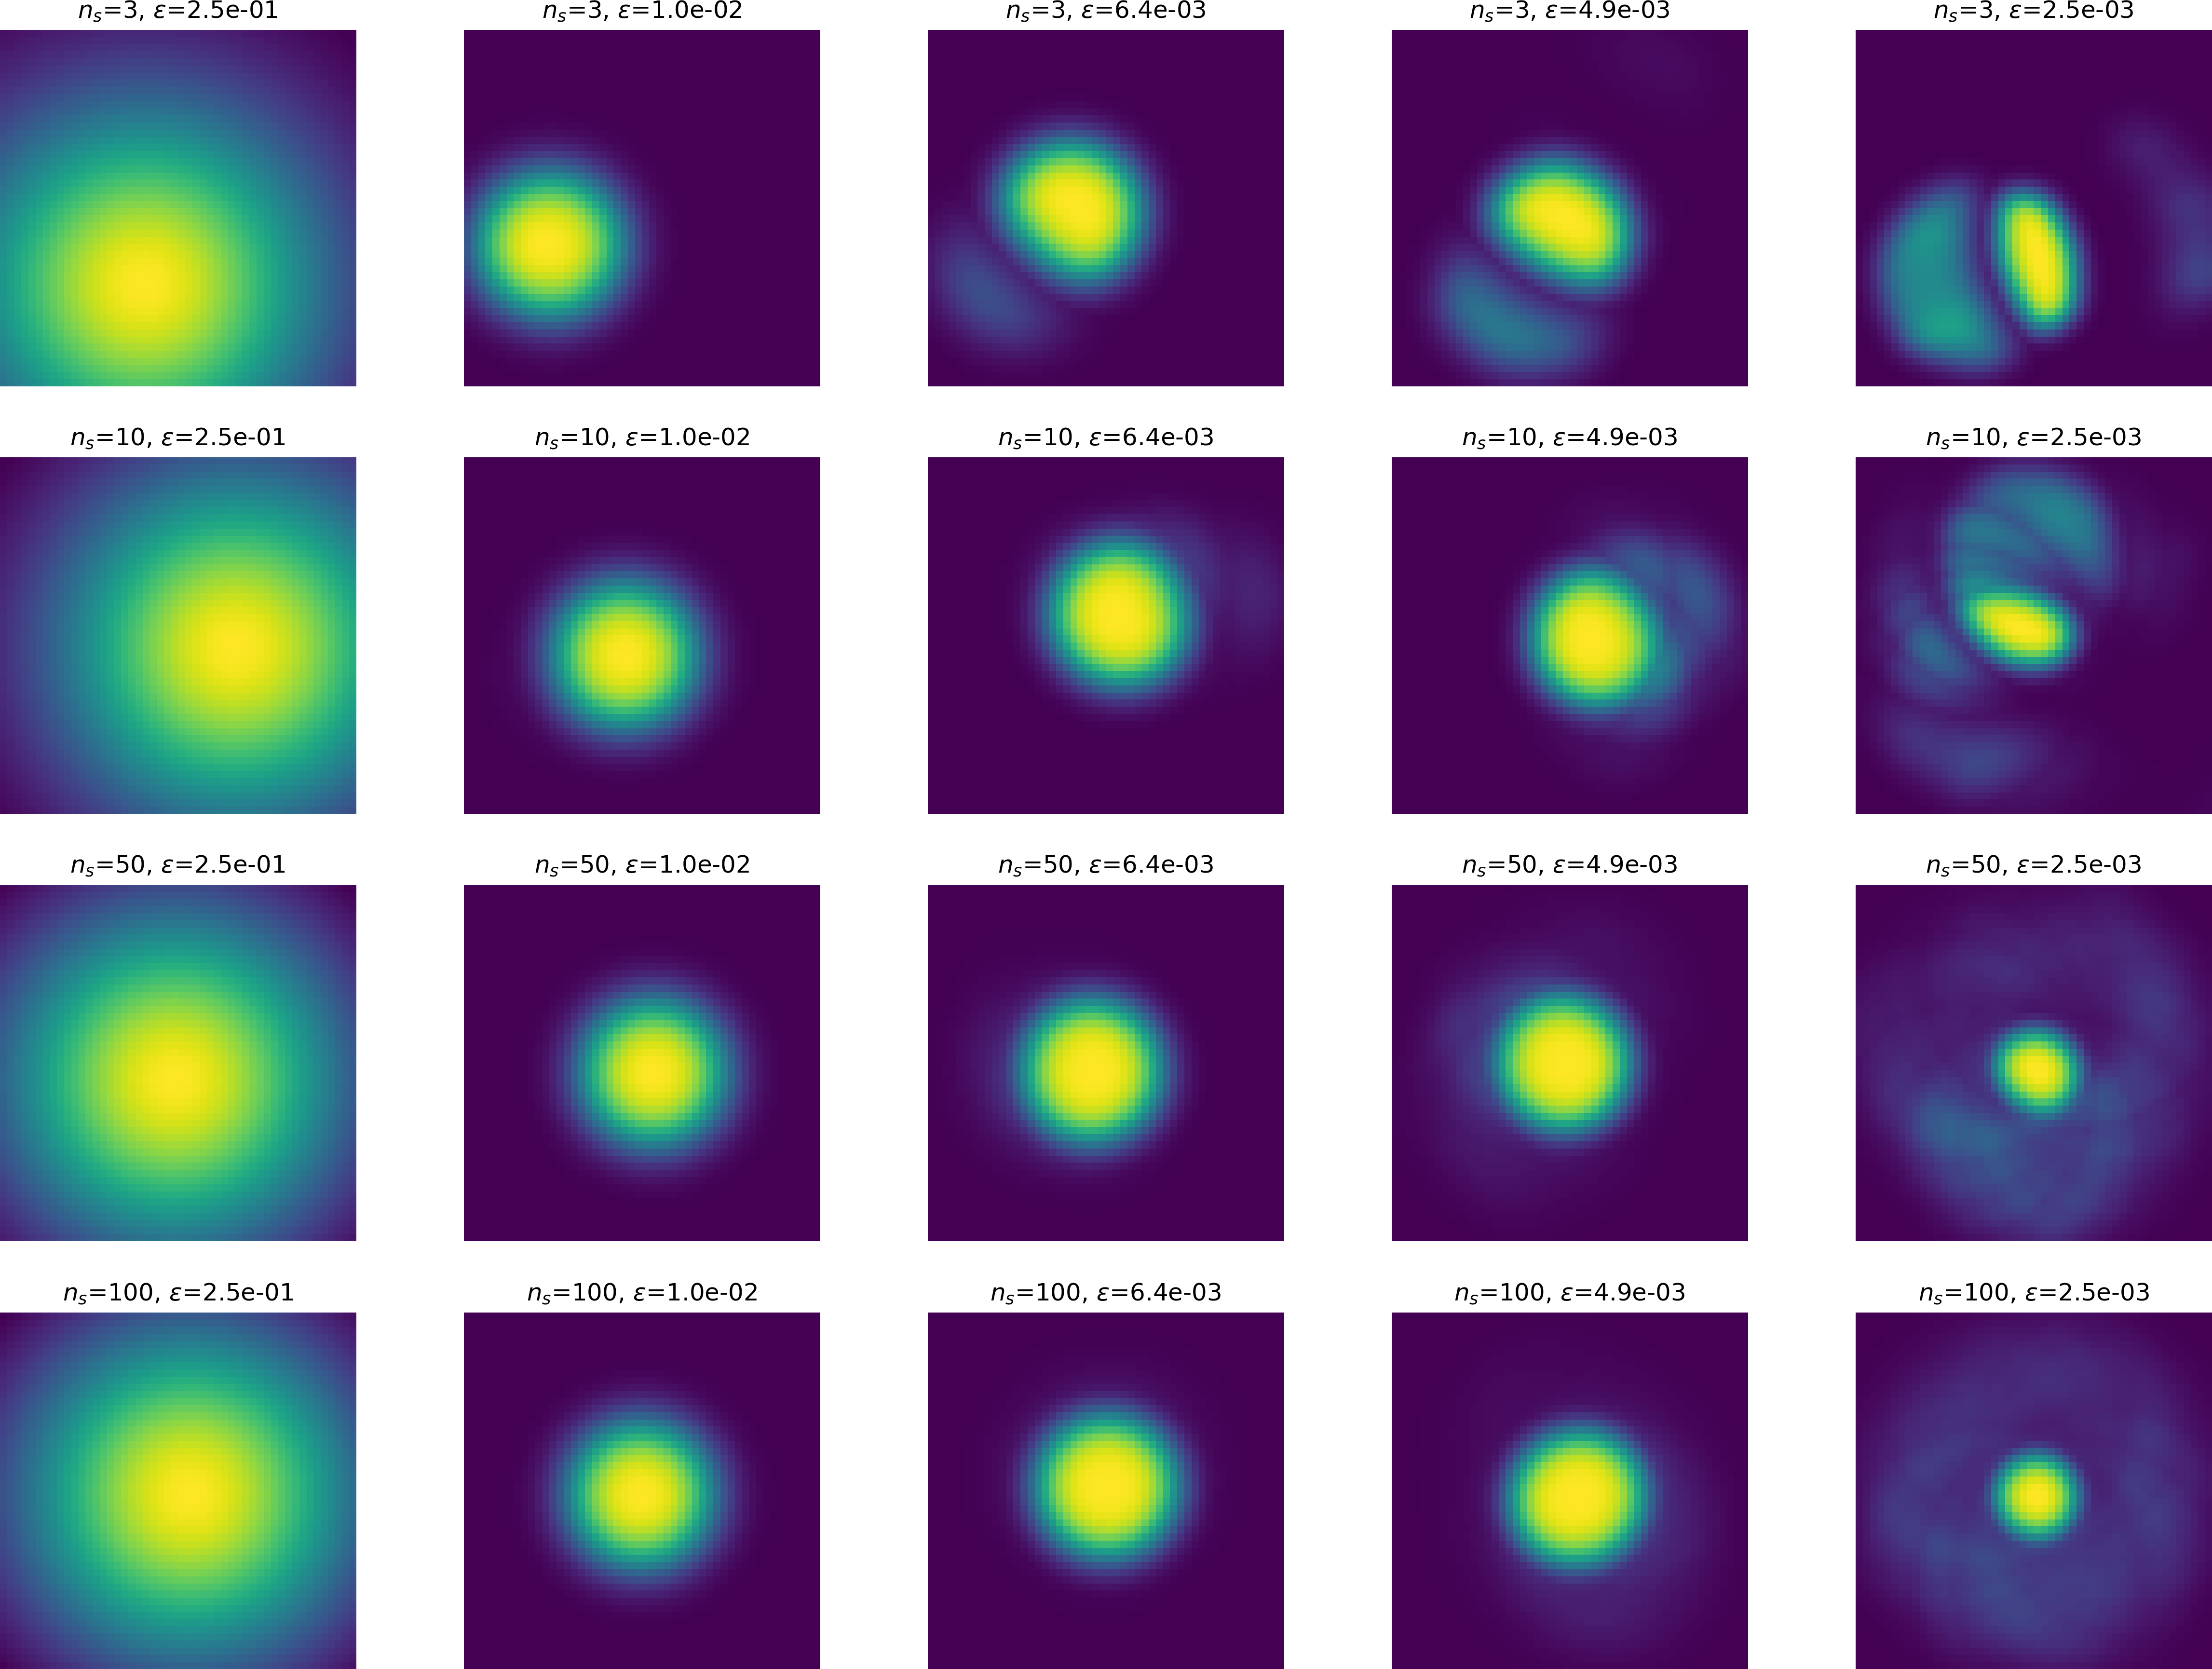
\includegraphics[width=.9\textwidth]{samples/2/all_circles.png}
    \caption{Barycenter of multiple sampled circles. On \textbf{rows} are varying number of samples $n_s$, ranging from $3$ to $100$. On columns are varying values of $\epsilon$, ranging from $0.5^2$ to $0.05^2$. Here, we see that the $L_2$ loss is not appropriate, because the mass is concentrated in the middle. Trying a dice score was not helping. A more intricate loss which would consider the support of half the mass could be better (refer to foot note on page \pageref{my_error}).}
    \label{fig:all_circles}
\end{figure}

\begin{figure}[p]
    \centering
    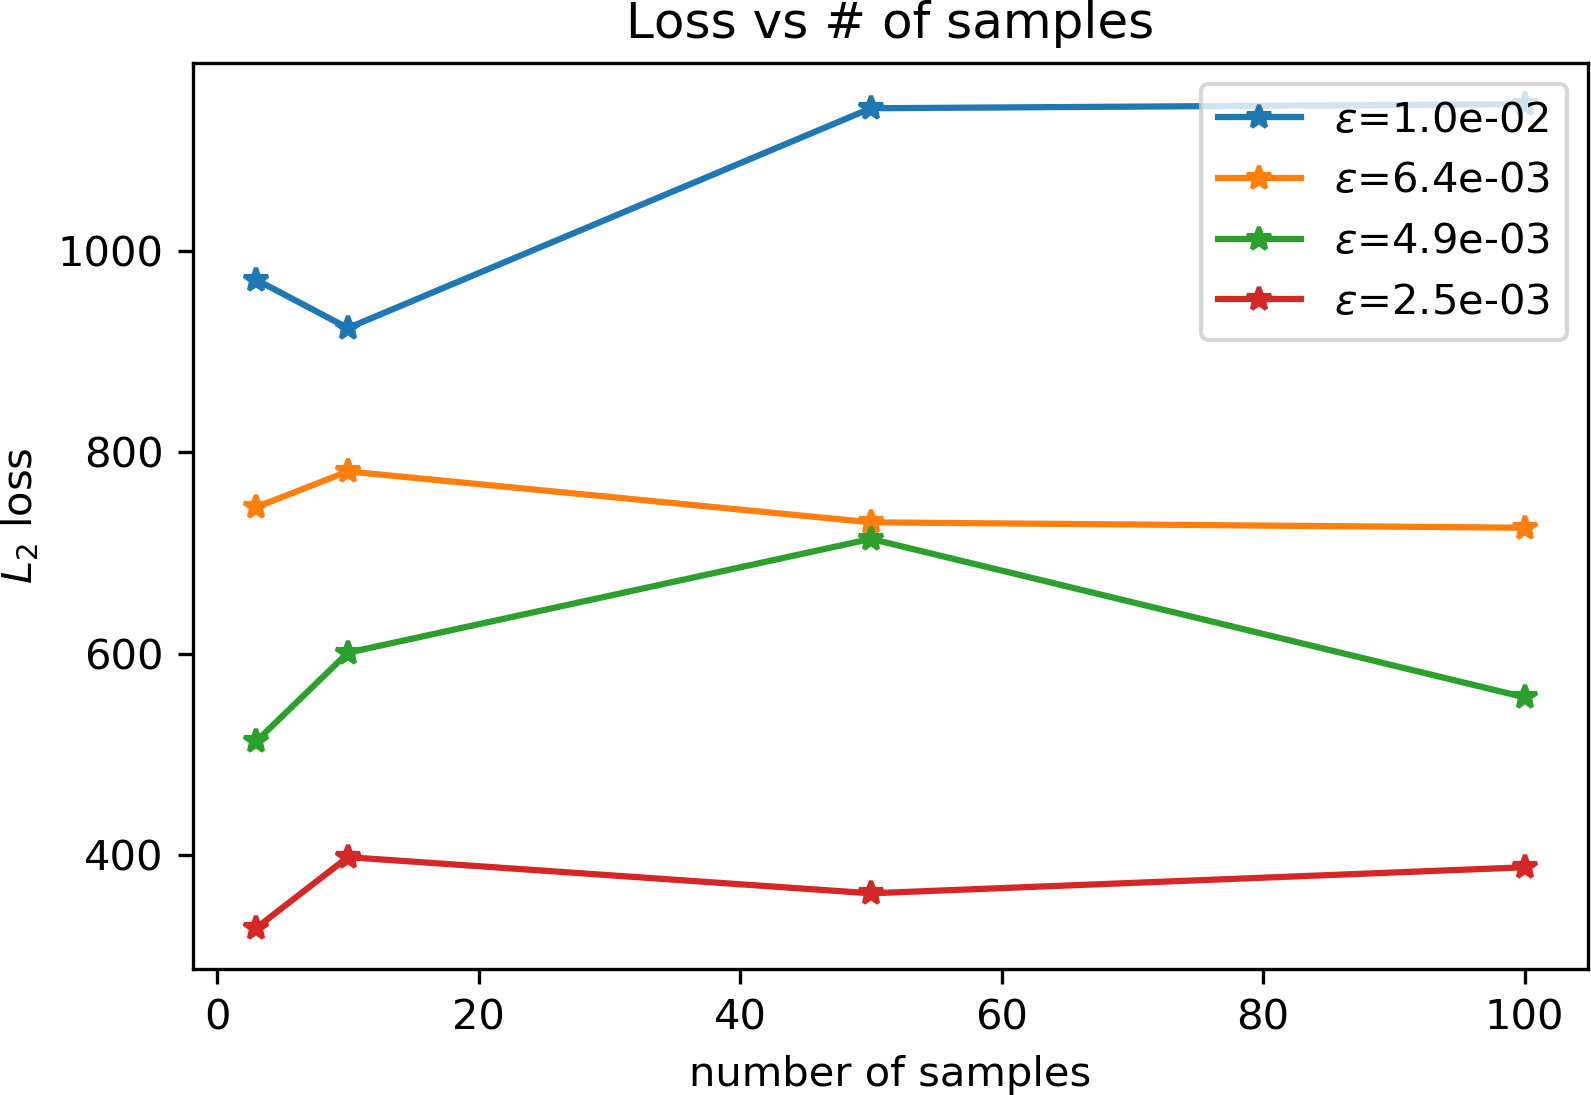
\includegraphics[width=.6\textwidth]{samples/2/l2_loss_brain.png}
    \caption{$L_2$ loss between the barycenter and the template, for the \textbf{phantom brains} dataset. As $\epsilon$ gets smaller, the barycenter becomes closer and closer to the expected template.}
    \label{fig:l2_loss_brain}
\end{figure}

\begin{figure}[p]
    \centering
    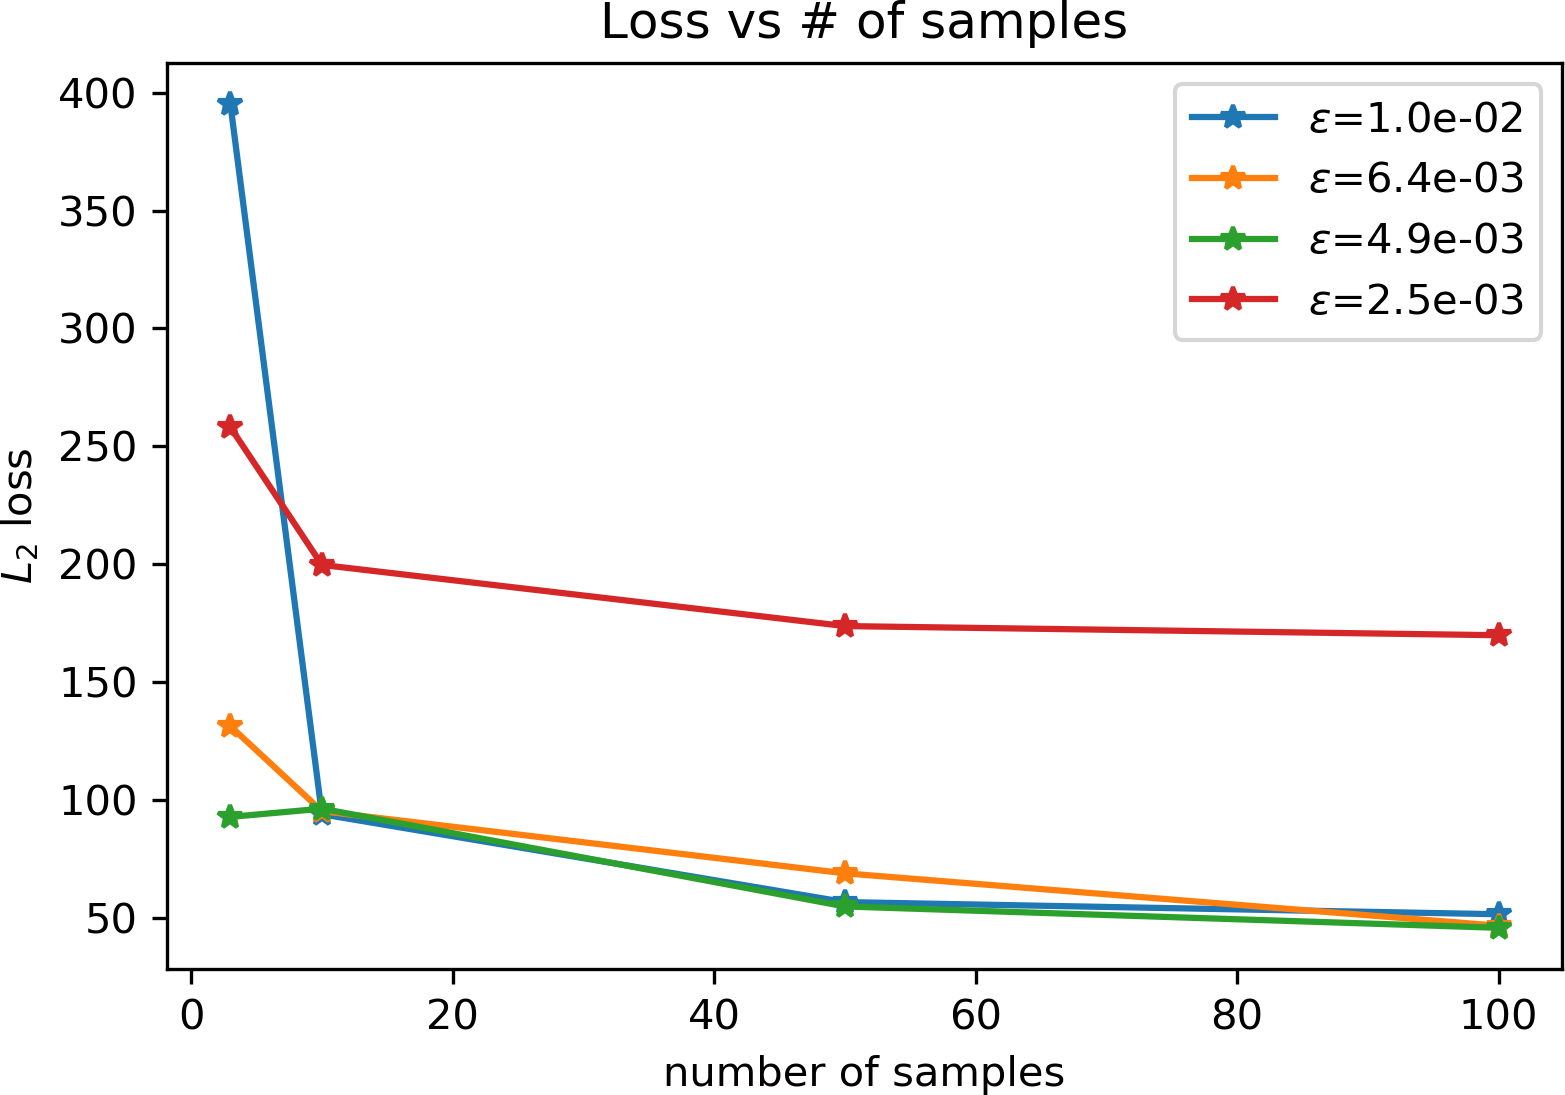
\includegraphics[width=.6\textwidth]{samples/2/l2_loss_circle.png}
    \caption{$L_2$ loss between the barycenter and the template, for the \textbf{circles} dataset. Here, we might be surprised that the loss does not decrease with the value of $\epsilon$. In fact, it's due to the $L_2$ loss being ill suited to measure the discrepancy between the images.}
    \label{fig:l2_loss_circle}
\end{figure}